\section{Pendahuluan}
\subsection{Latar Belakang}
Pada Wireless Jaringan Komputer, terdapat setidaknya 3 jenis, yaitu Point-to-Point Protocol
(PPP), Point-to-multipoint dan Wireless Bridging.\\\\
Point-to-Point Protocol (PPP) adalah data link protokol yang umum digunakan dalam
membangun hubungan langsung antara dua node jaringan. Hal ini dapat menyediakan koneksi
otentikasi, transmisi enkripsi (menggunakan ECP, RFC 1968), dan kompresi. Jenis ini
biasanya digunakan untuk menghubungkan jaringan antar 2 gedung atau antar 2 BTS (Base
Transceiver Station).\\\\
Point-to-multipoint adalah pendekatan yang paling populer untuk komunikasi nirkabel yang
memiliki banyak node, tujuan akhir atau pengguna akhir. Jenis ini biasanya digunakan untuk
membuat wifi atau hotspot yang berasal dari 1 sumber disebar ke banyak client dalam suatu
jaringan.\\\\
Wireless Bridging digunakan untuk menghubungkan dua segmen LAN melalui tautan
nirkabel. Kedua segmen akan berada di subnet yang sama dan terlihat seperti dua switch
Ethernet yang dihubungkan oleh kabel ke semua komputer di subnet.\\\\
Untuk mengembangkan jaringan komputer berbasis wireless yang berkualitas dan mempunyai
ketersediaan tinggi, penggunaan 3 jenis ini perlu disesuaikan dengan kebutuhan dan kondisi
nya, sehingga kali ini saya akan membahasnya 1 persatu dari 3 jenis koneksi wireless
tersebut.

\subsection{Maksud dan Tujuan}
Mengetahui dan memahami 3 jenis koneksi pada Jaringan Wireless.

\subsection{Hasil yang diharapkan}
Dapat mengkonfigurasi koneksi Wireless Bridge, Point to Point dan Point to Multipoint
dengan tepat.

%===========================================================%
\section{Tugas Pendahuluan}
\begin{enumerate}
	\item Buatlah topologi jaringan percobaan 1, 2, dan 3!
	\item Perbedaan Point-to-Point, Point-to-Multipoint, dan Wireless Bridging
	\item Follow IG Lab MIOT
\end{enumerate}

%===========================================================%
\section{Alat dan Bahan}
\begin{itemize}[label=$\bullet$, itemsep=-1pt, leftmargin=*]
	\item 2 atau lebih perangkat router mikrotik yang sudah support wireless.
	\item Aplikasi Winbox.
\end{itemize}

%===========================================================%
\section{Jangka Waktu Pelaksanaan}
Pemahaman dan konfigurasi 1 jam.

%===========================================================%
\section{Proses dan Tahapan Konfigurasi}
%======================PERCOBAAN 1==========================%
\subsection{Wireless Point to Point}
Untuk koneksi Point to Point seperti contohnya topologi seperti dibawah ini, biasanya
digunakan untuk menghubungkan 2 router atau 2 node jaringan, Hal ini dilakukan biasanya
untuk koneksi koneksi jarak jauh yang mengharapkan kecepatan tinggi misal untuk
menghubungkan jaringan antar gedung, menghubungkan BTS (Base Transceiver Station) to
BTS (Base Transceiver Station). Koneksi point to point ini akan lebih aman karena maksimal
node yang terhubung hanya 2. Untuk konfigurasinya seperti berikut ini.

\begin{center}
	\textbf{Konfigurasi Router 1}
	\begin{enumerate}
		\item Buka aplikasi WinBox pada PC 1 dan lakukan koneksi ke Router 1.\\Neighbors > Refresh > Double click Router yang terdeteksi > Connect
		\begin{figure}[H]
			\centering
			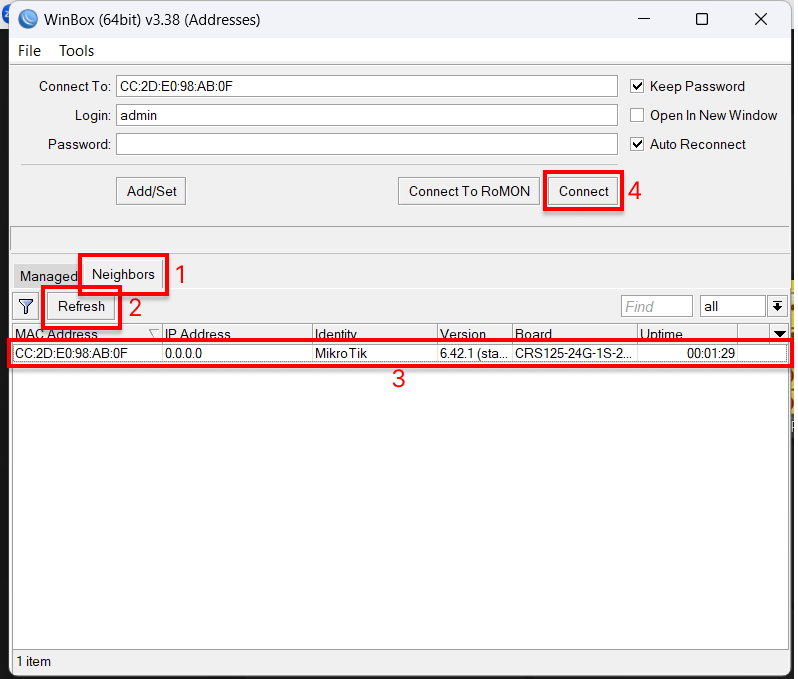
\includegraphics[width=0.8\linewidth]{P1/img/per1/pc1/Step 1.png}
			\caption{Step 1}
			\label{fig:Step 1(Per.1 PC1)}
		\end{figure}
		\item Berikan IP address pada interface wlan 1 yang dapat dibuat pada tab IP > Addresses.
		\begin{figure}[H]
			\centering
			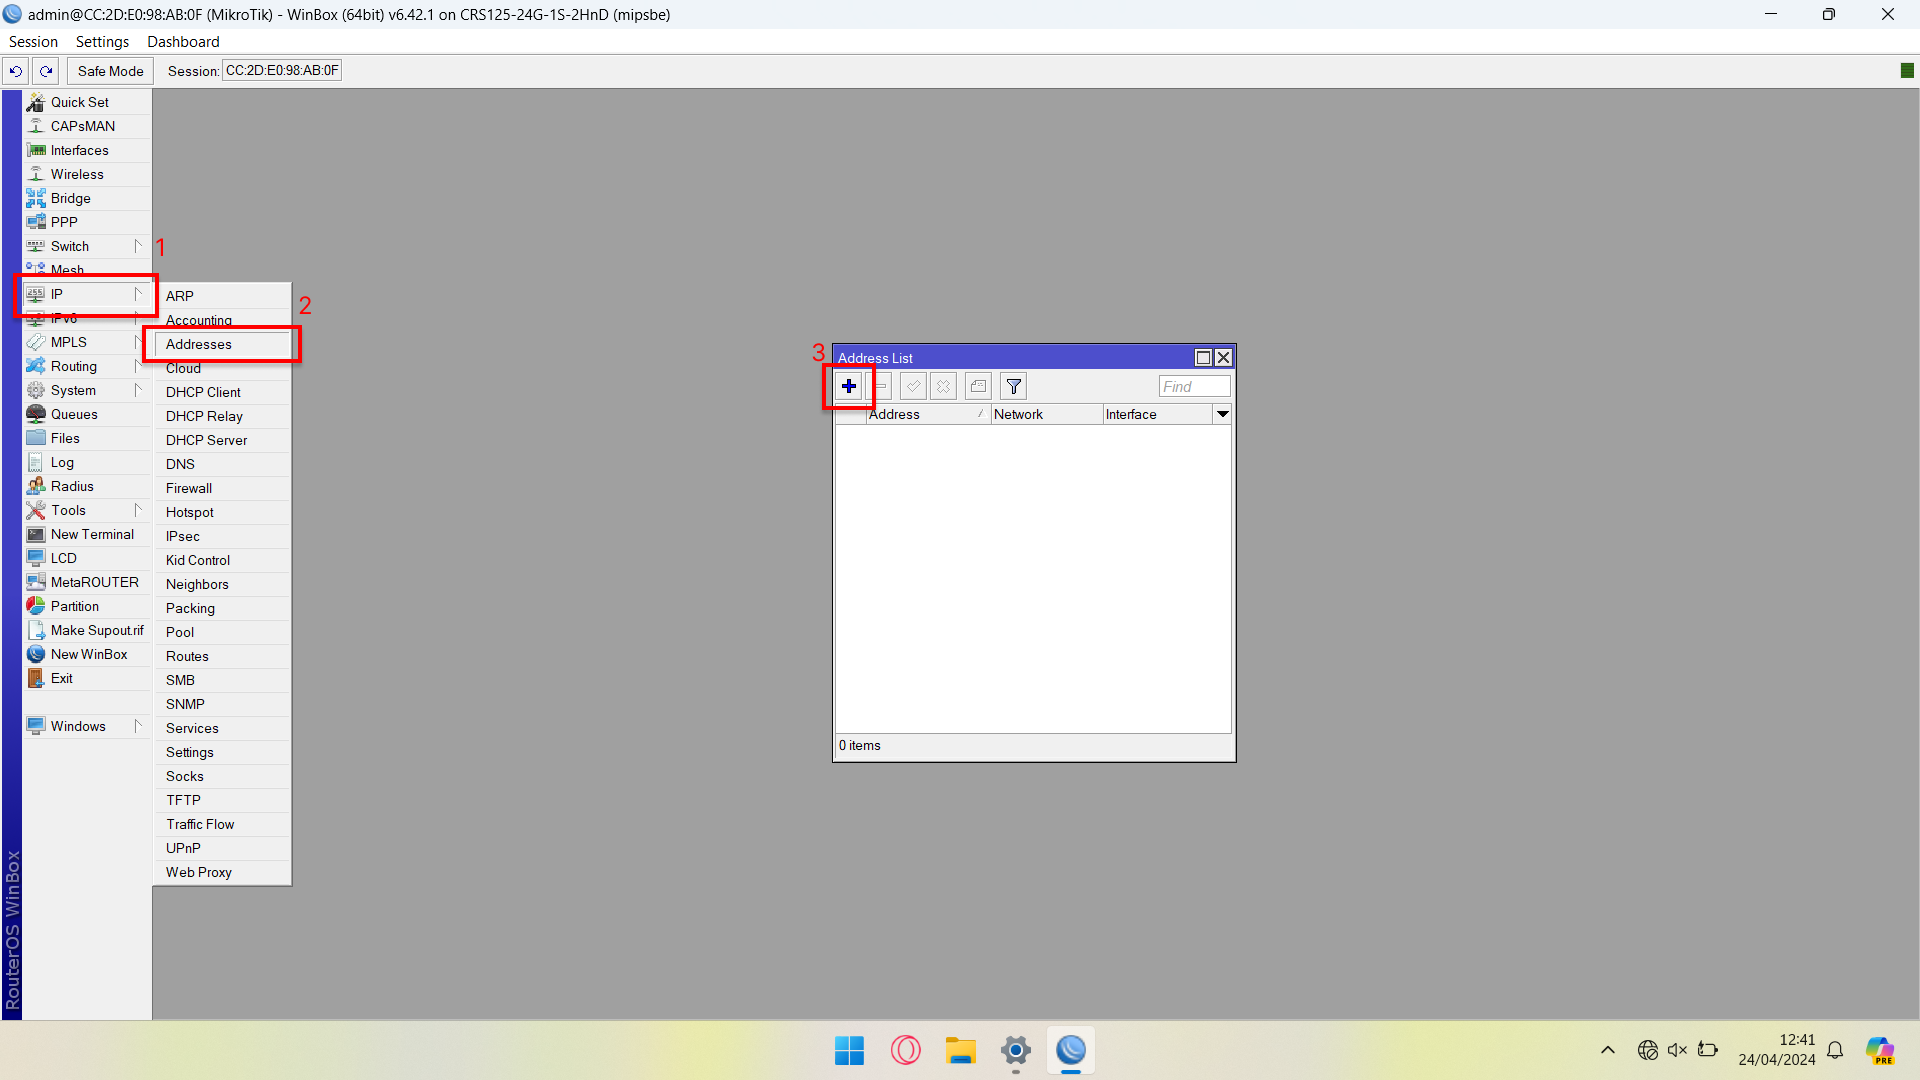
\includegraphics[width=0.9\linewidth]{P1/img/per1/pc1/Step 2.1.png}
			\caption{Step 2.1}
			\label{fig:Step 2.1(Per.1 PC1)}
		\end{figure}
		\item Berikan IP address sesuai dengan cara pengaturan IP address yang benar. Berikan IP address yang berbeda dengan contoh di modul.
		\begin{figure}[H]
			\centering
			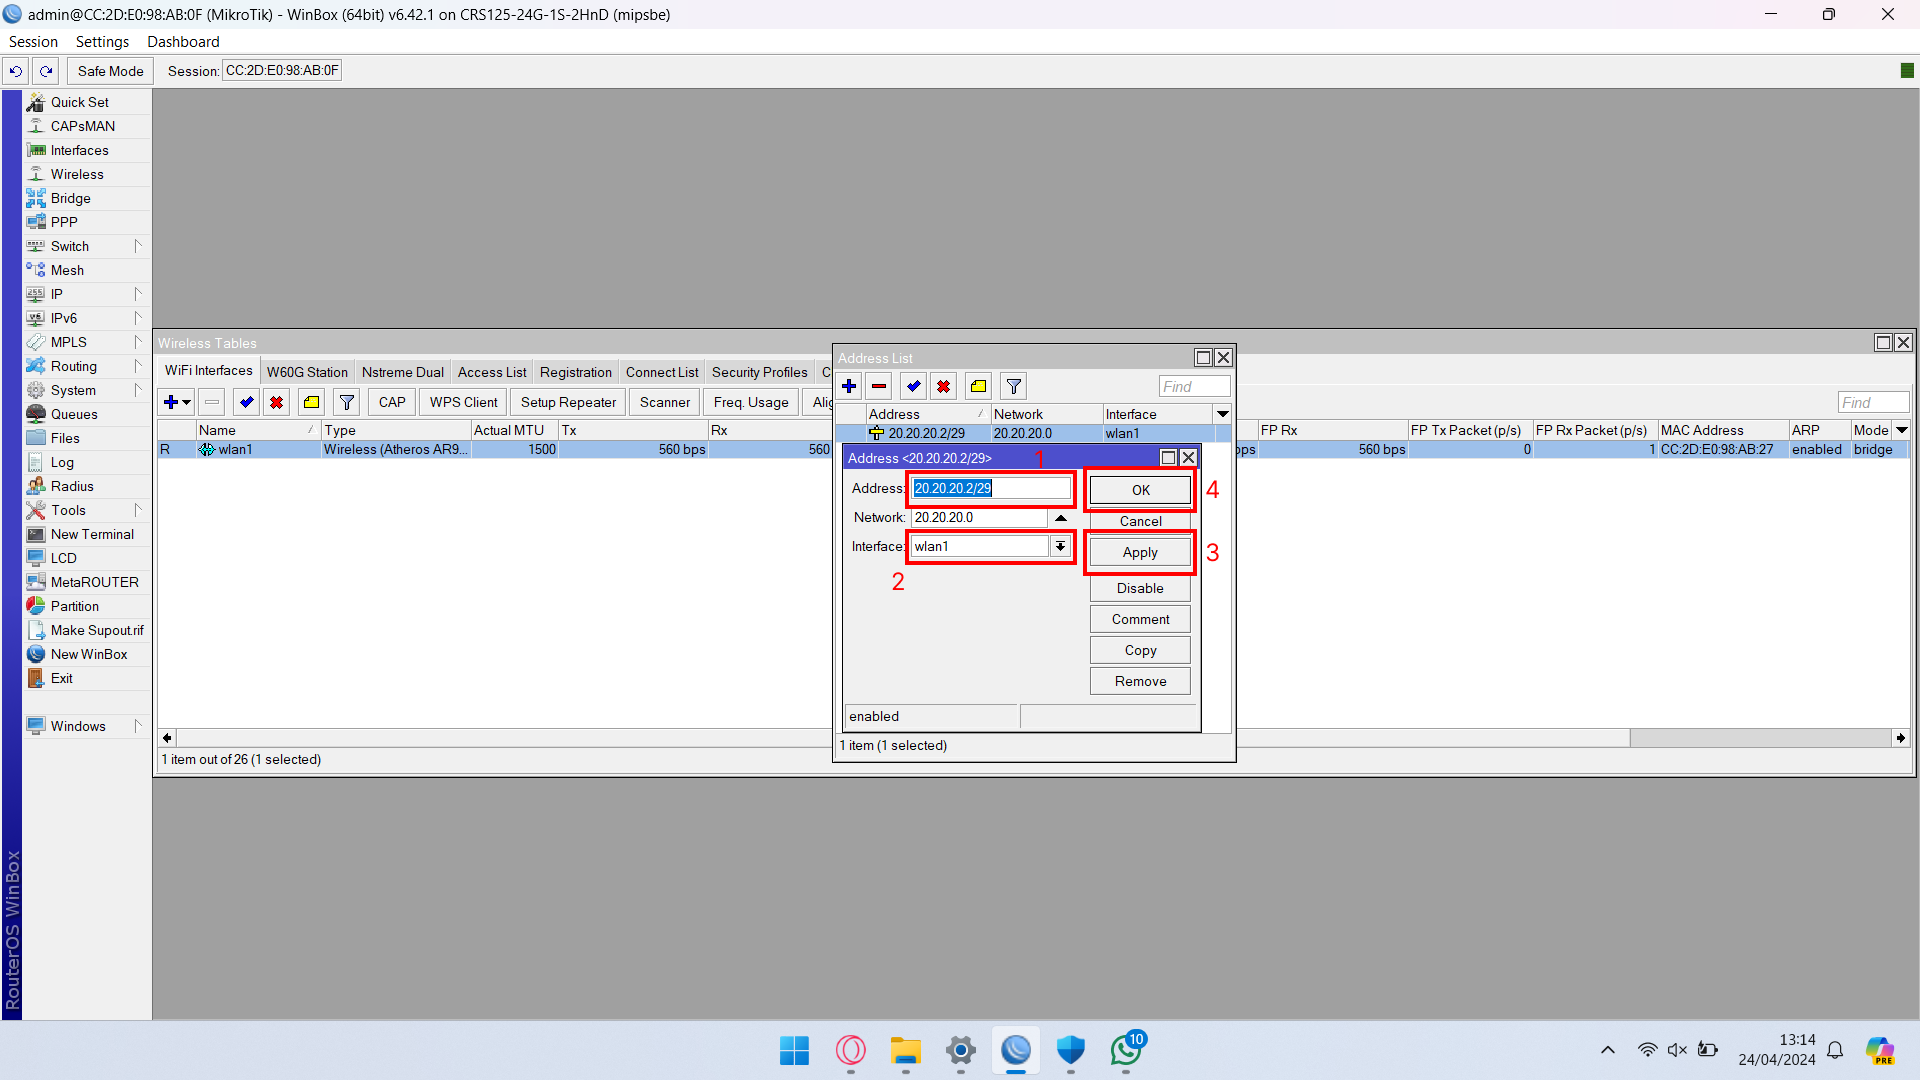
\includegraphics[width=0.9\linewidth]{P1/img/per1/pc1/Step 2.2.png}
			\caption{Step 2.2}
			\label{fig:Step 2.2(Per.1 PC1)}
		\end{figure}
		\item Atur Router 1 untuk mengaktifkan WLAN pada tab Wireless, pilih wlan1, lalu klik tombol centang. Kemudian atur WLAN pada mode bridge dan isi SSID yang diinginkan. Berikan SSID sekreatif mungkin, yang berbeda dengan contoh di modul.
		\begin{figure}[H]
			\centering
			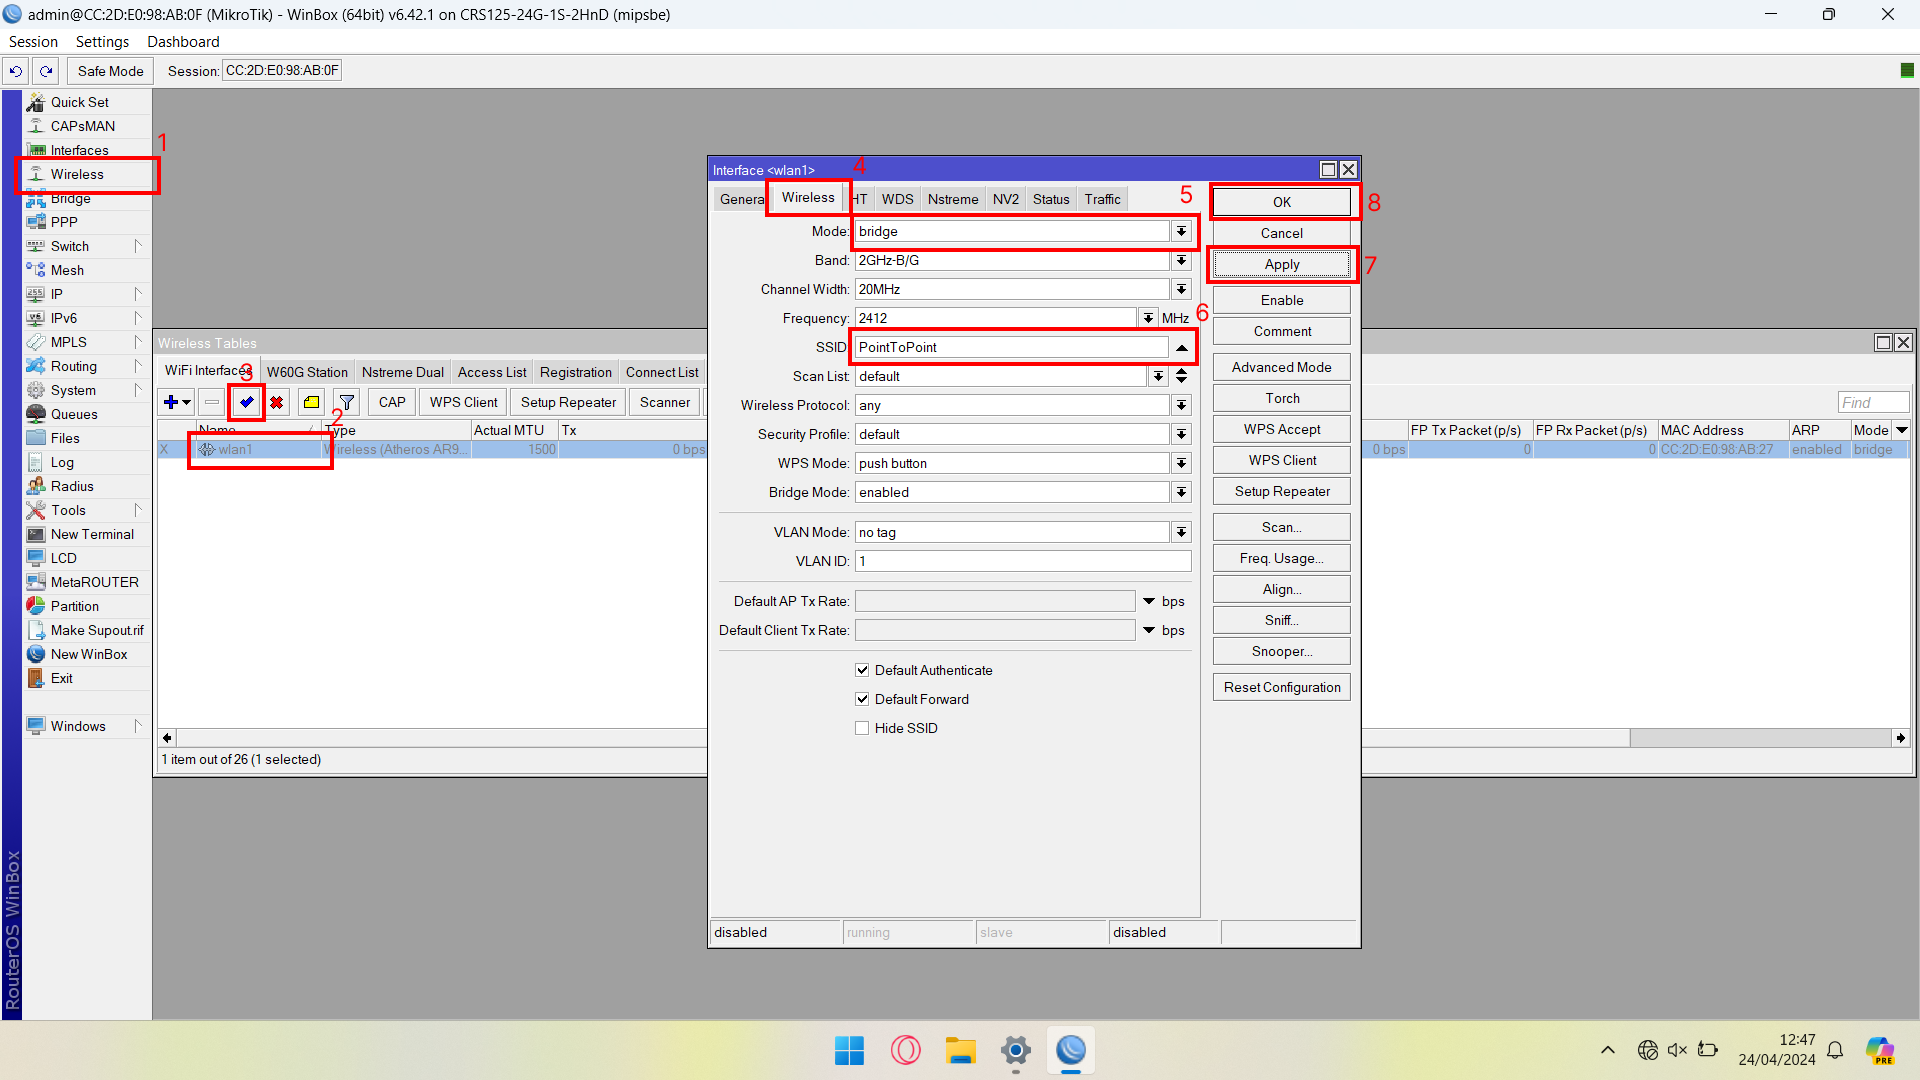
\includegraphics[width=0.9\linewidth]{P1/img/per1/pc1/Step 3.png}
			\caption{Step 3}
			\label{fig:Step 3(Per.1 PC1)}
		\end{figure}
	\end{enumerate}
	 
	\textbf{Konfigurasi Router 2}
	\begin{enumerate}
		\item Buka WinBox dan lakukan koneksi ke Router
		\item Berikan IP address pada interface wlan 1 yang dapat dibuat pada tab IP > Addresses. Berikan IP address sesuai dengan cara pengaturan IP address yang benar. Berikan IP address yang berbeda dengan contoh di modul.
		\begin{figure}[H]
			\centering
			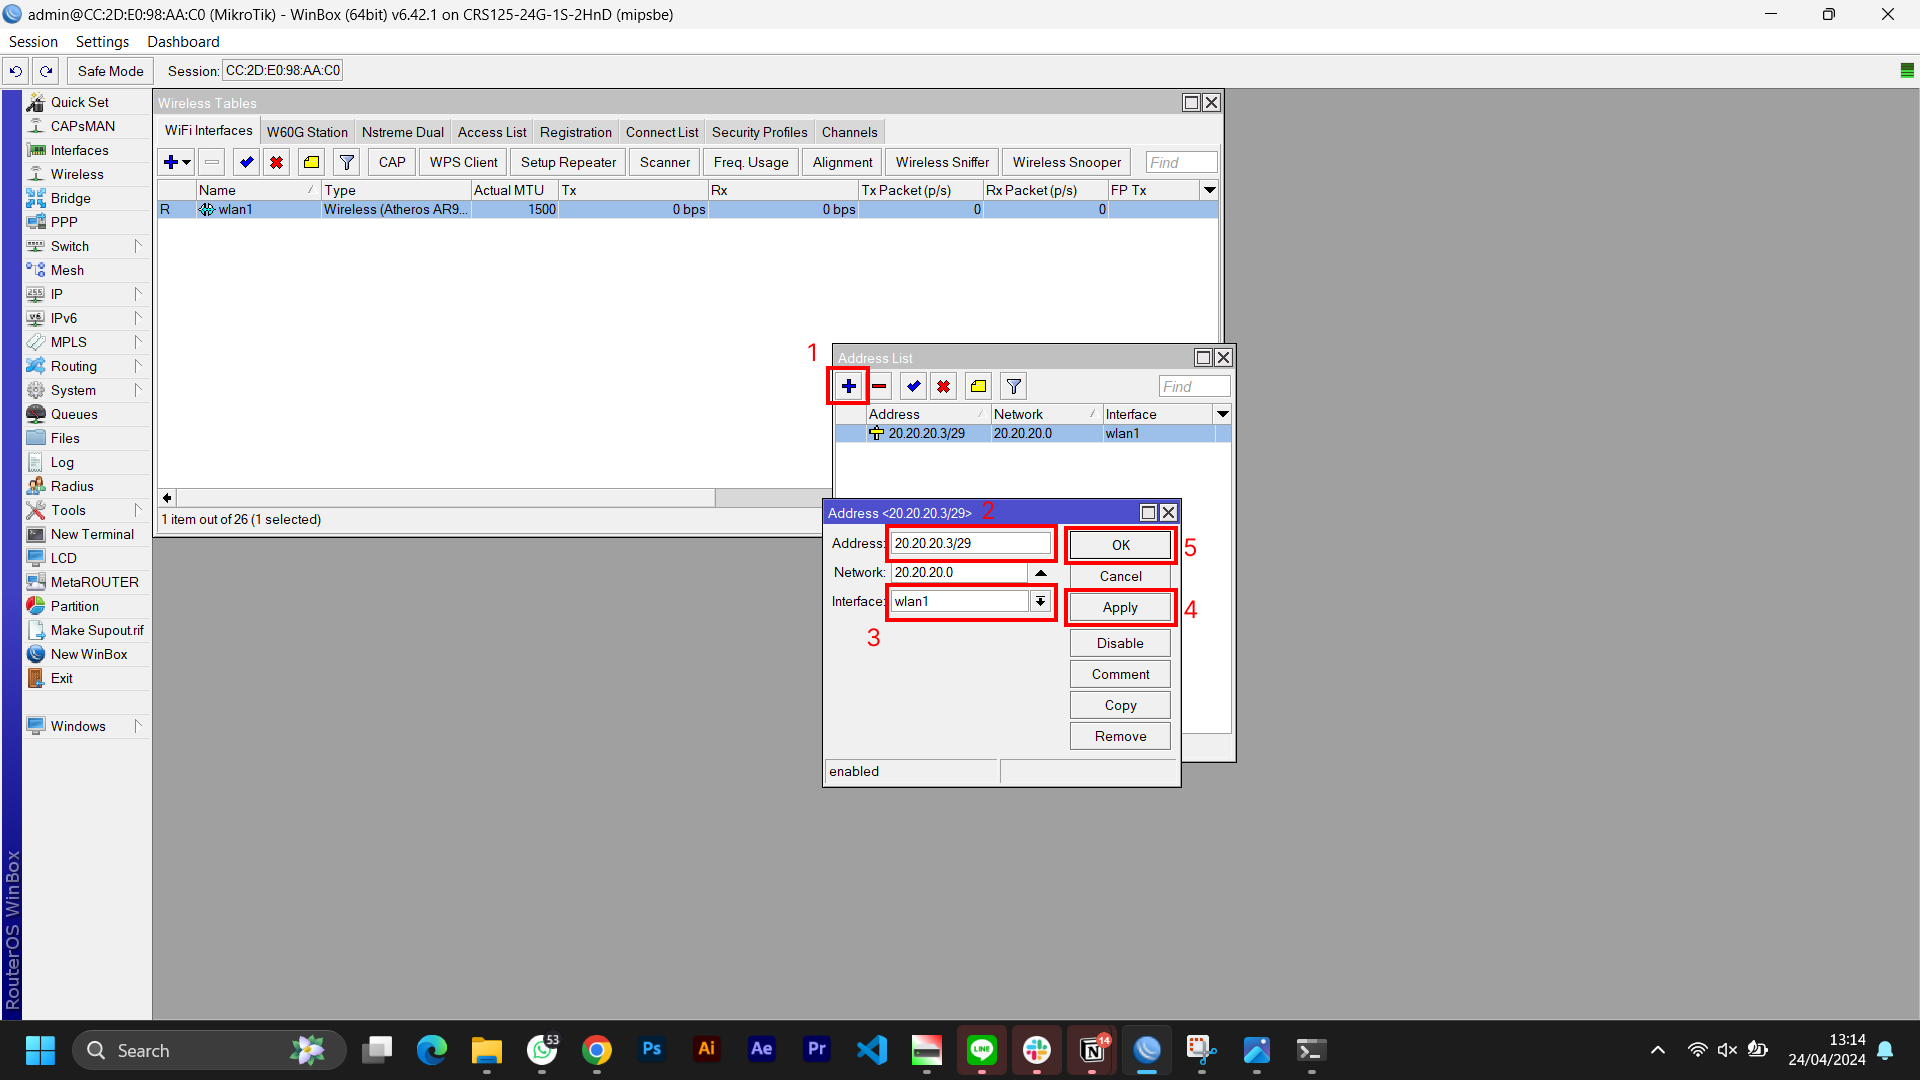
\includegraphics[width=0.9\linewidth]{P1/img/per1/pc2/Step 2.png}
			\caption{Step 2}
			\label{fig:Step 2(Per.1 PC2)}
		\end{figure}
		\item Atur Router 2 untuk mengaktifkan WLAN pada tab Wireless, pilih wlan1, lalu klik tombol centang. Kemudian atur WLAN pada mode station. Kemudian cari sinyal yang sudah dipancarkan oleh Router 1, sesuai dengan nama SSID yang sudah dibuat
		\begin{figure}[H]
			\centering
			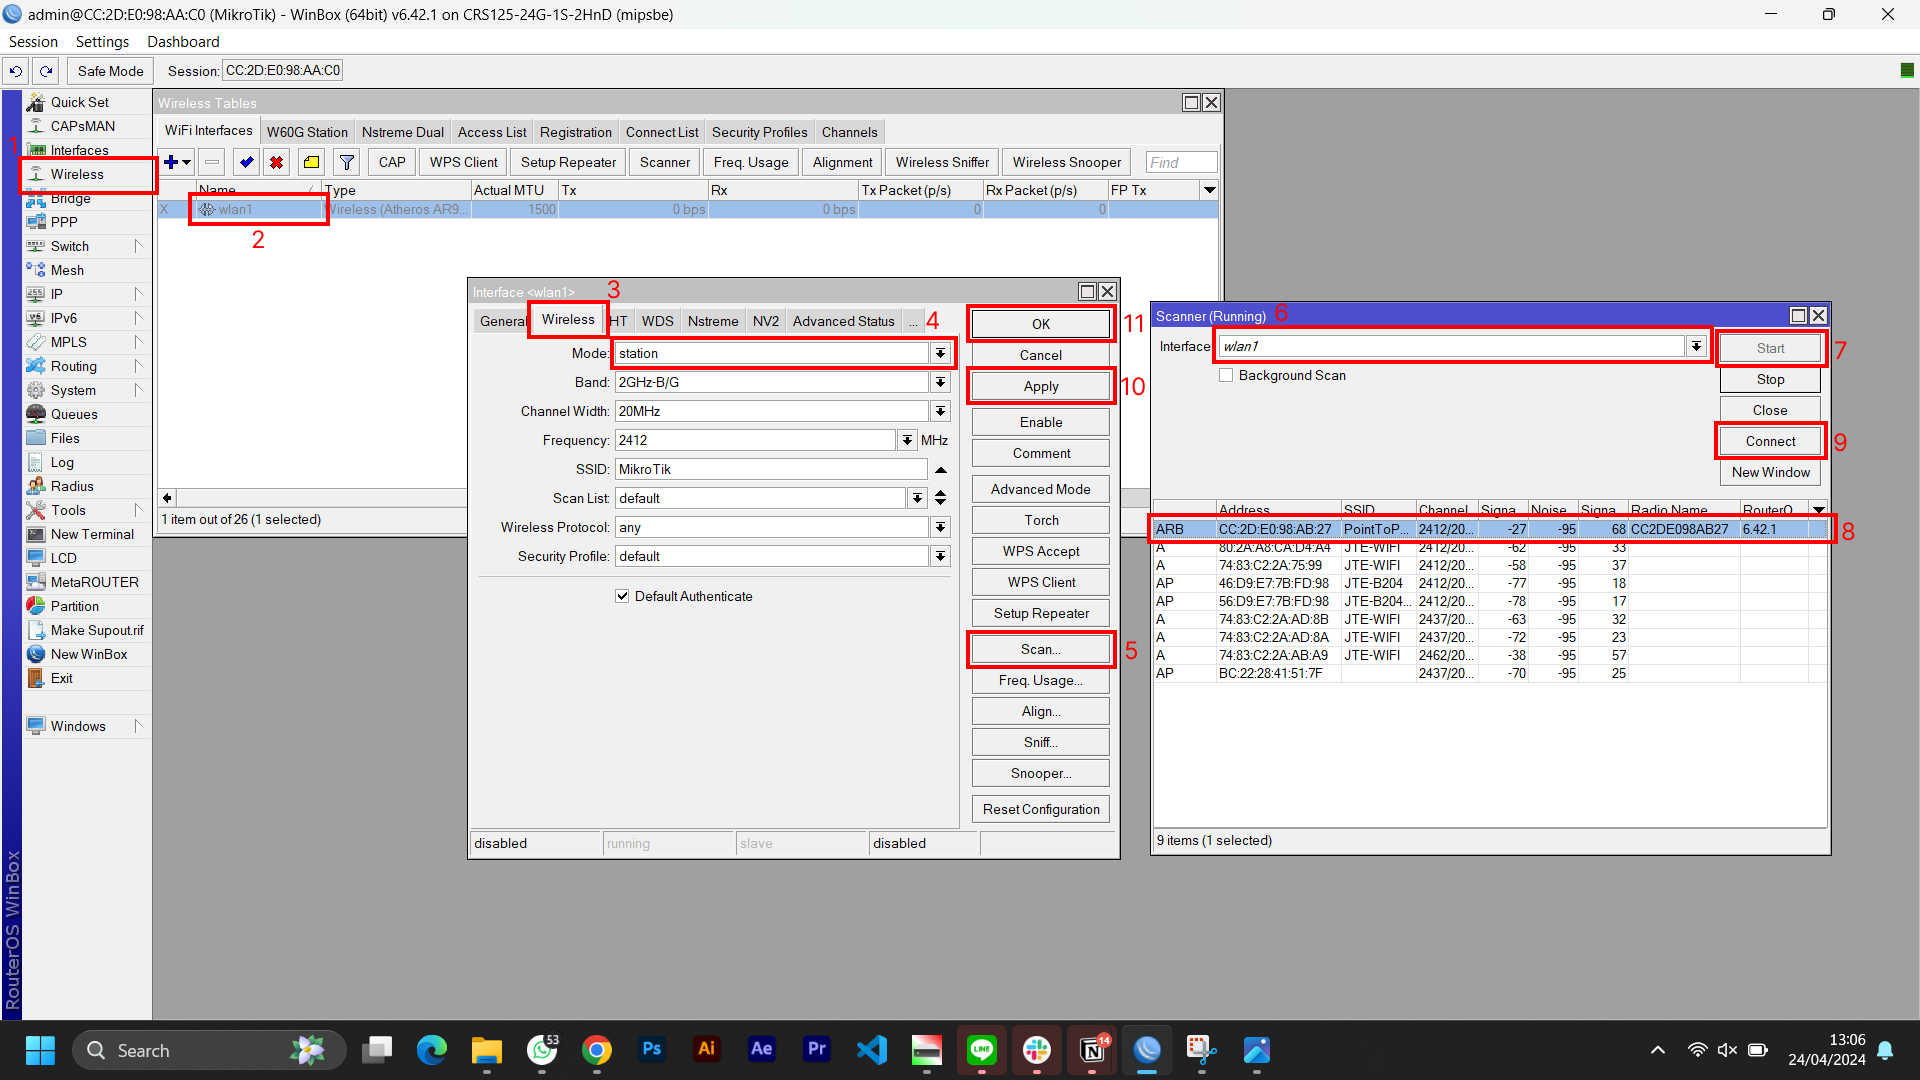
\includegraphics[width=0.9\linewidth]{P1/img/per1/pc2/Step 3.png}
			\caption{Step 3}
			\label{fig:Step 3(Per.1 PC2)}
		\end{figure}
	\end{enumerate}
	                              
	\textbf{Mengecek keberhasilan konfigurasi}
	\begin{enumerate}
		\item Lakukan test ping dari Router 1 ke Router 2
		\begin{figure}[H]
			\centering
			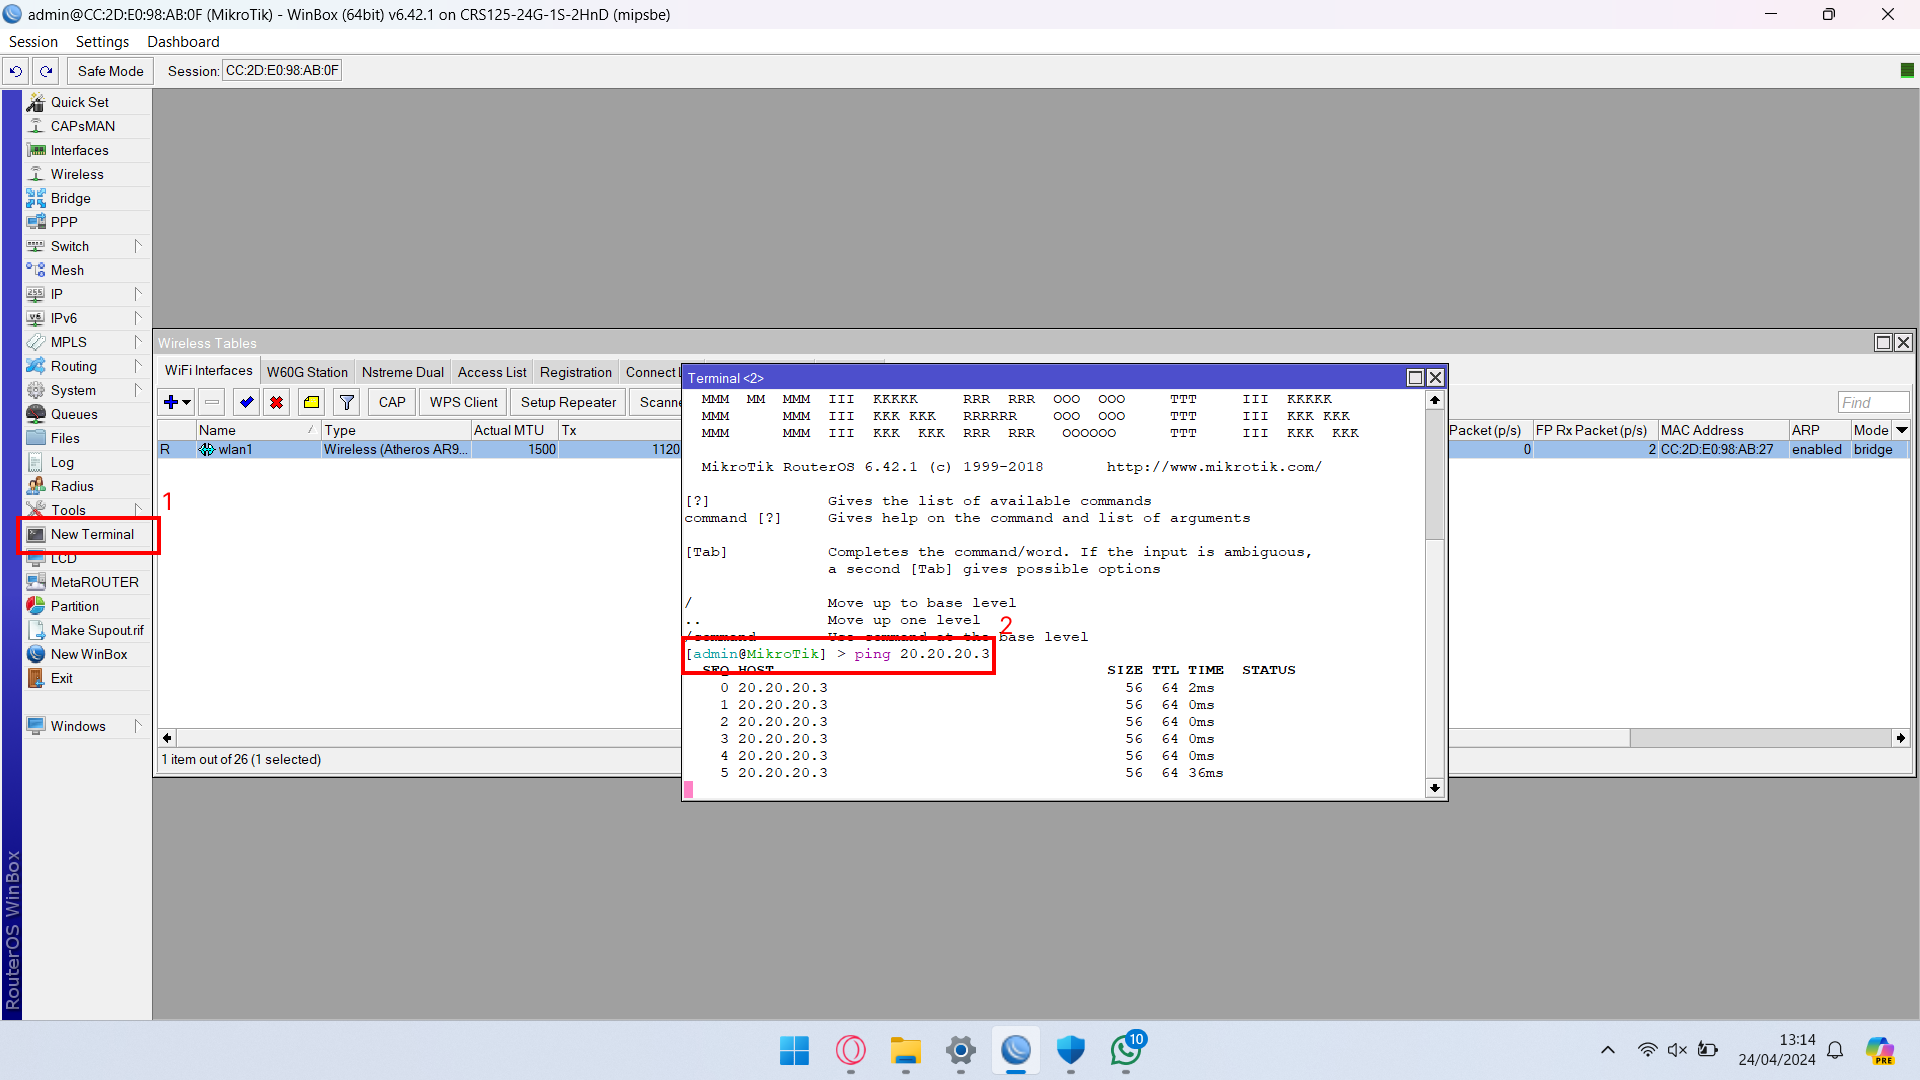
\includegraphics[width=0.9\linewidth]{P1/img/per1/pc1/Step 4.png}
			\caption{Step 1}
			\label{fig:Ping Step 1(Per.1 PC1)}
		\end{figure}
		\item Lakukan test ping dari Router 2 ke Router 1
		\begin{figure}[H]
			\centering
			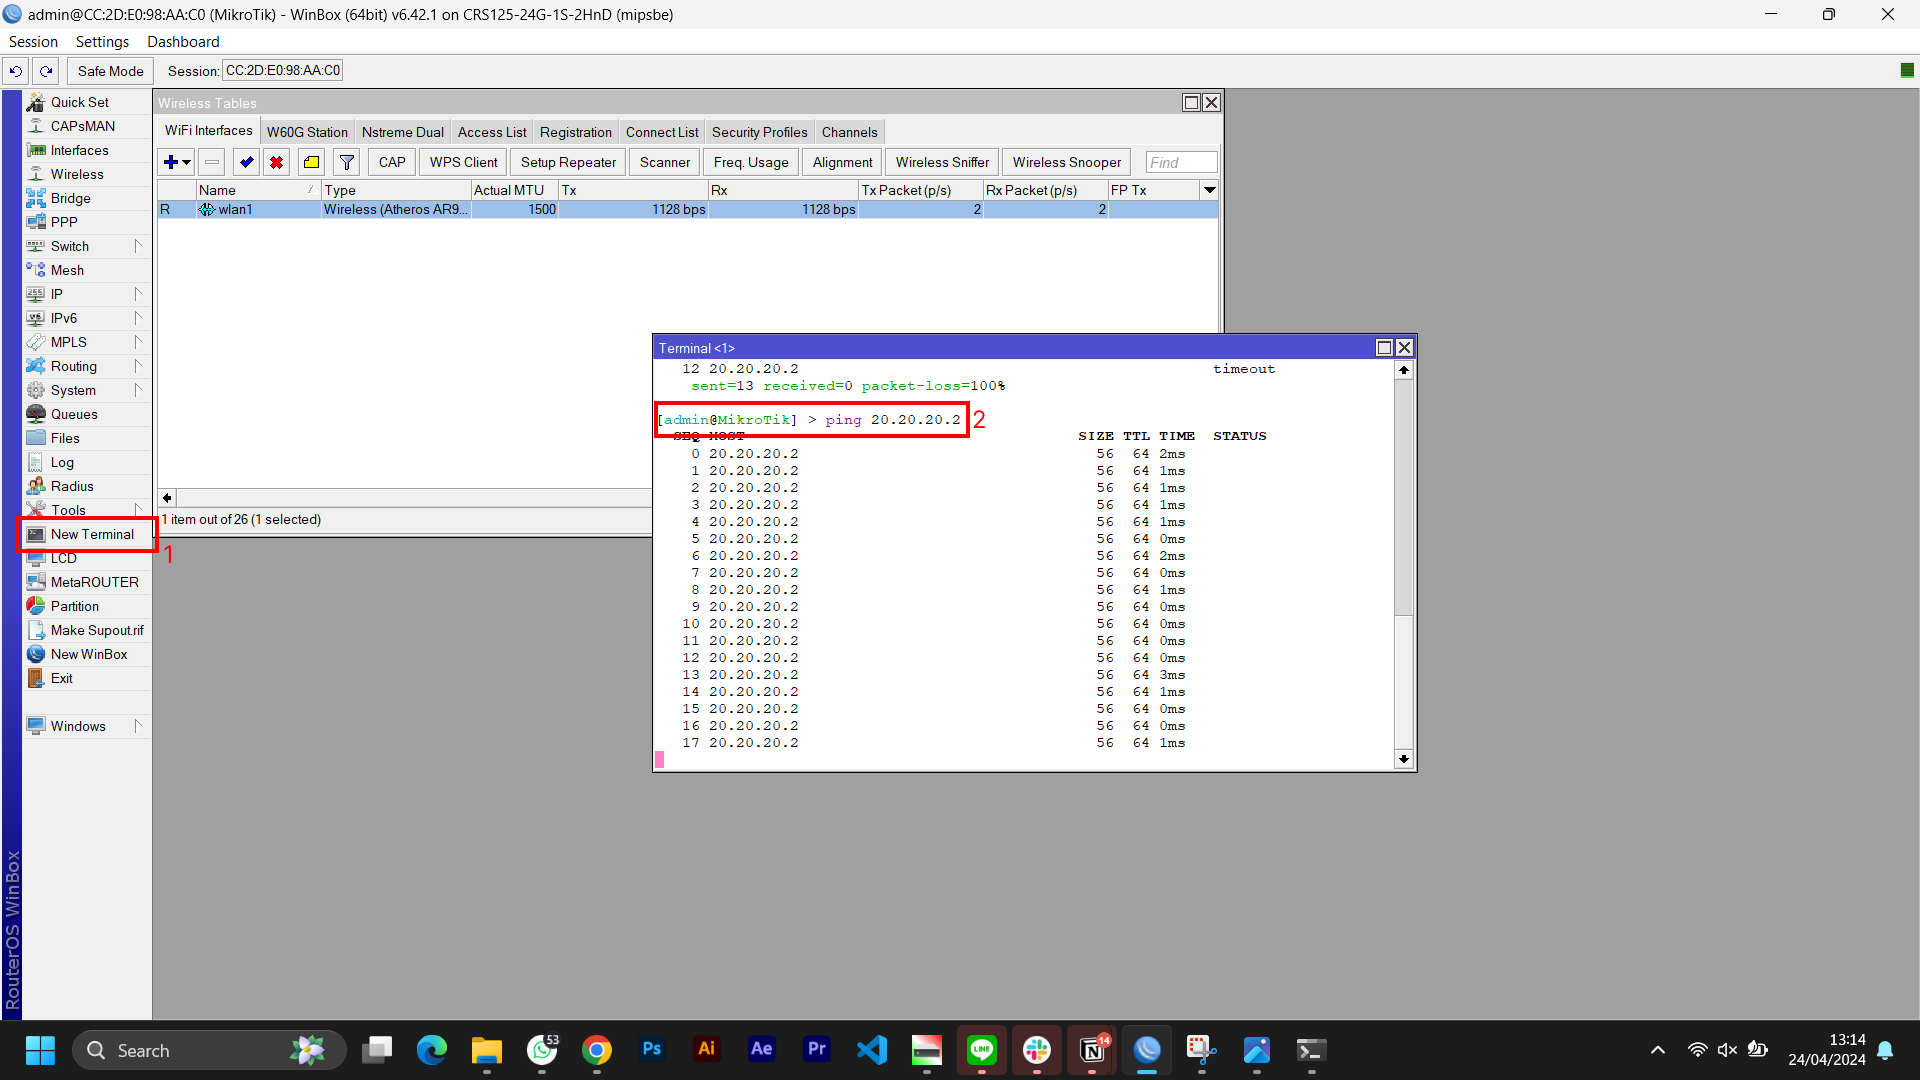
\includegraphics[width=0.9\linewidth]{P1/img/per1/pc2/Step 4.png}
			\caption{Step 2}
			\label{fig:Ping Step 2(Per.1 PC2)}
		\end{figure}
	\end{enumerate}
\end{center}

%======================PERCOBAAN 2==========================%
\subsection{Wireless Point to Multipoint}
Koneksi ini yang paling banyak digunakan, karena kelebihannya yaitu dapat mengkoneksikan
multipoint atau banyak node dari satu point atau node sumber, penerapan pada koneksi ini
biasanya berupa hotspot. Untuk konfigurasinya seperti berikut.
Untuk gambar topologi sama dengan PointToPoint, hanya saja berbeda di konfigurasi dan
mode pada routernya.
\begin{center}
	\textbf{Konfigurasi Router 1}
	\begin{enumerate}
		\item Berikan IP address sesuai dengan cara pengaturan IP address yang benar. Berikan IP address yang berbeda dengan contoh di modul.
		\begin{figure}[H]
			\centering
			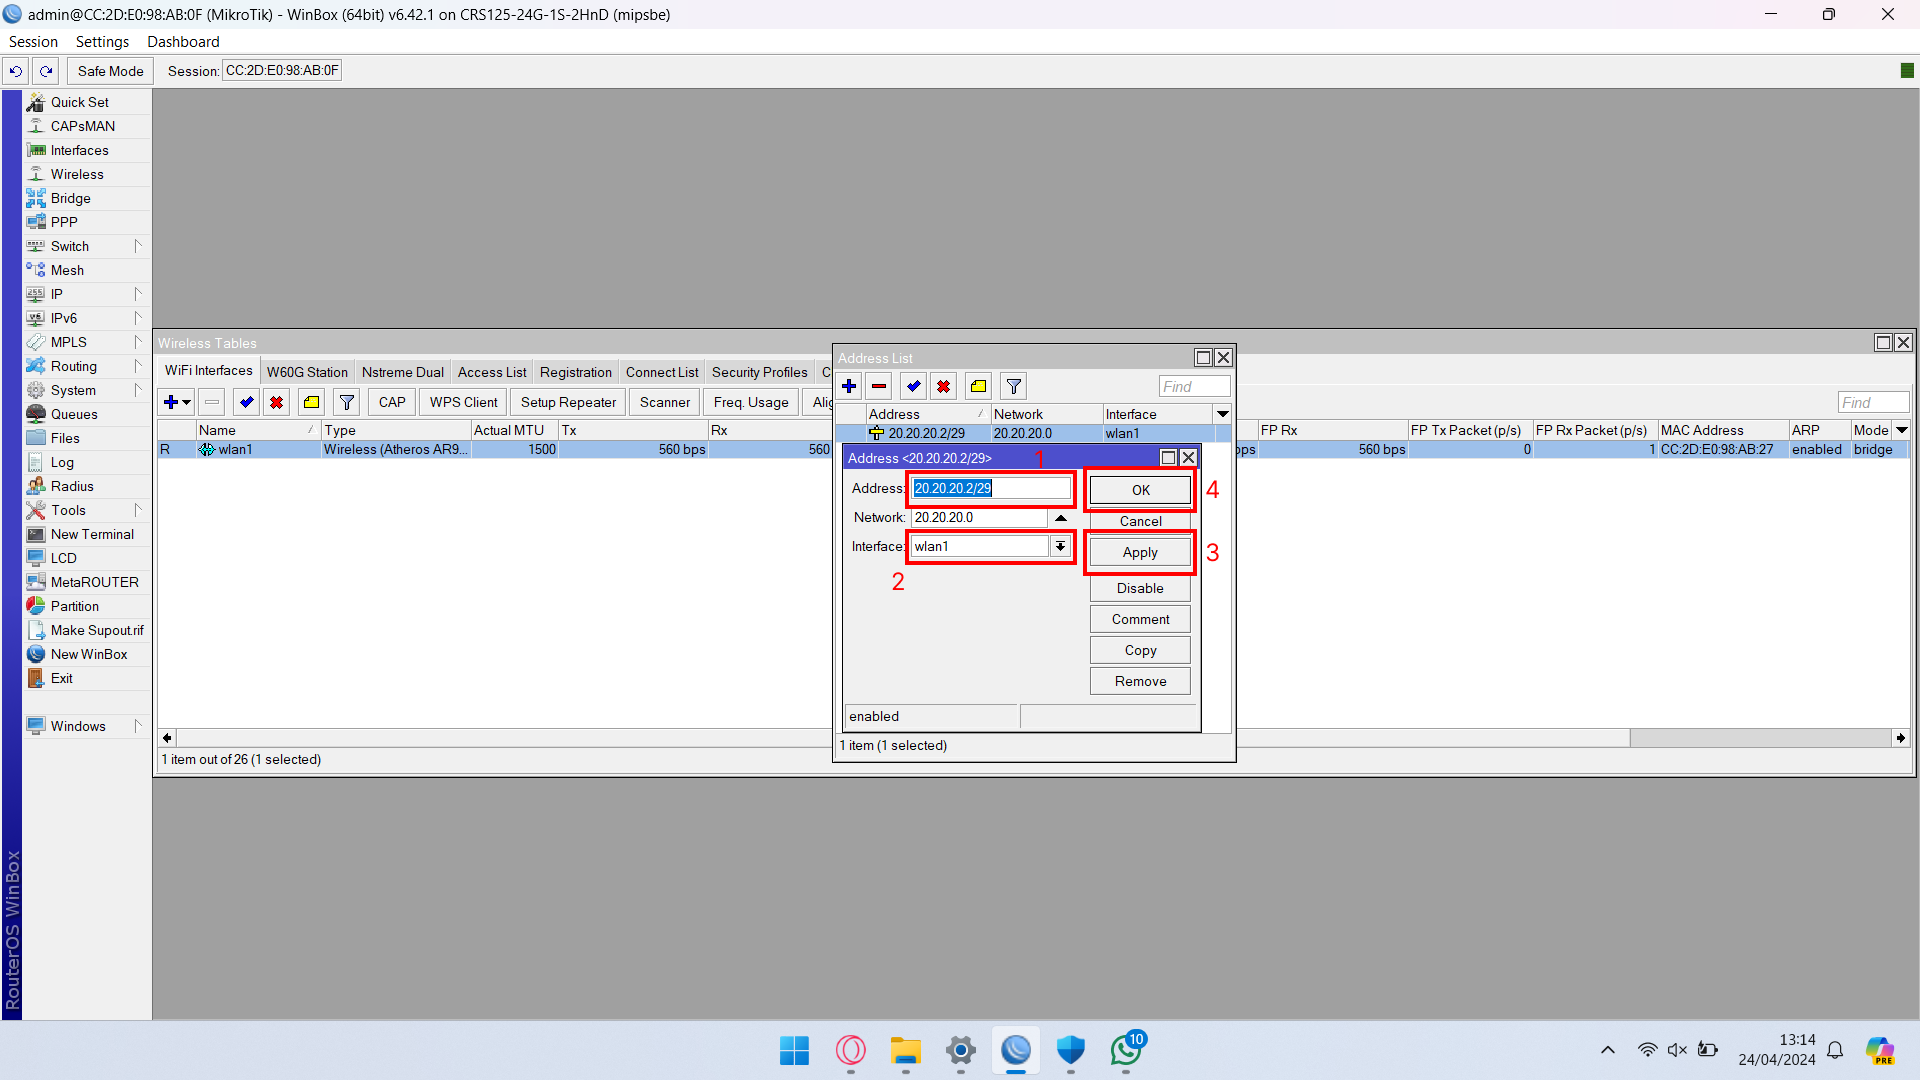
\includegraphics[width=0.9\linewidth]{P1/img/per1/pc1/Step 2.2.png}
			\caption{Step 1}
			\label{fig:Step 1(Per.2 PC1)}
		\end{figure}
		\item Atur Router 1 untuk mengaktifkan WLAN pada tab Wireless, pilih wlan1, lalu klik tombol centang. Kemudian atur WLAN pada mode ap bridge dan isi SSID yang diinginkan. Berikan SSID sekreatif mungkin, yang berbeda dengan contoh di modul.
		\begin{figure}[H]
			\centering
			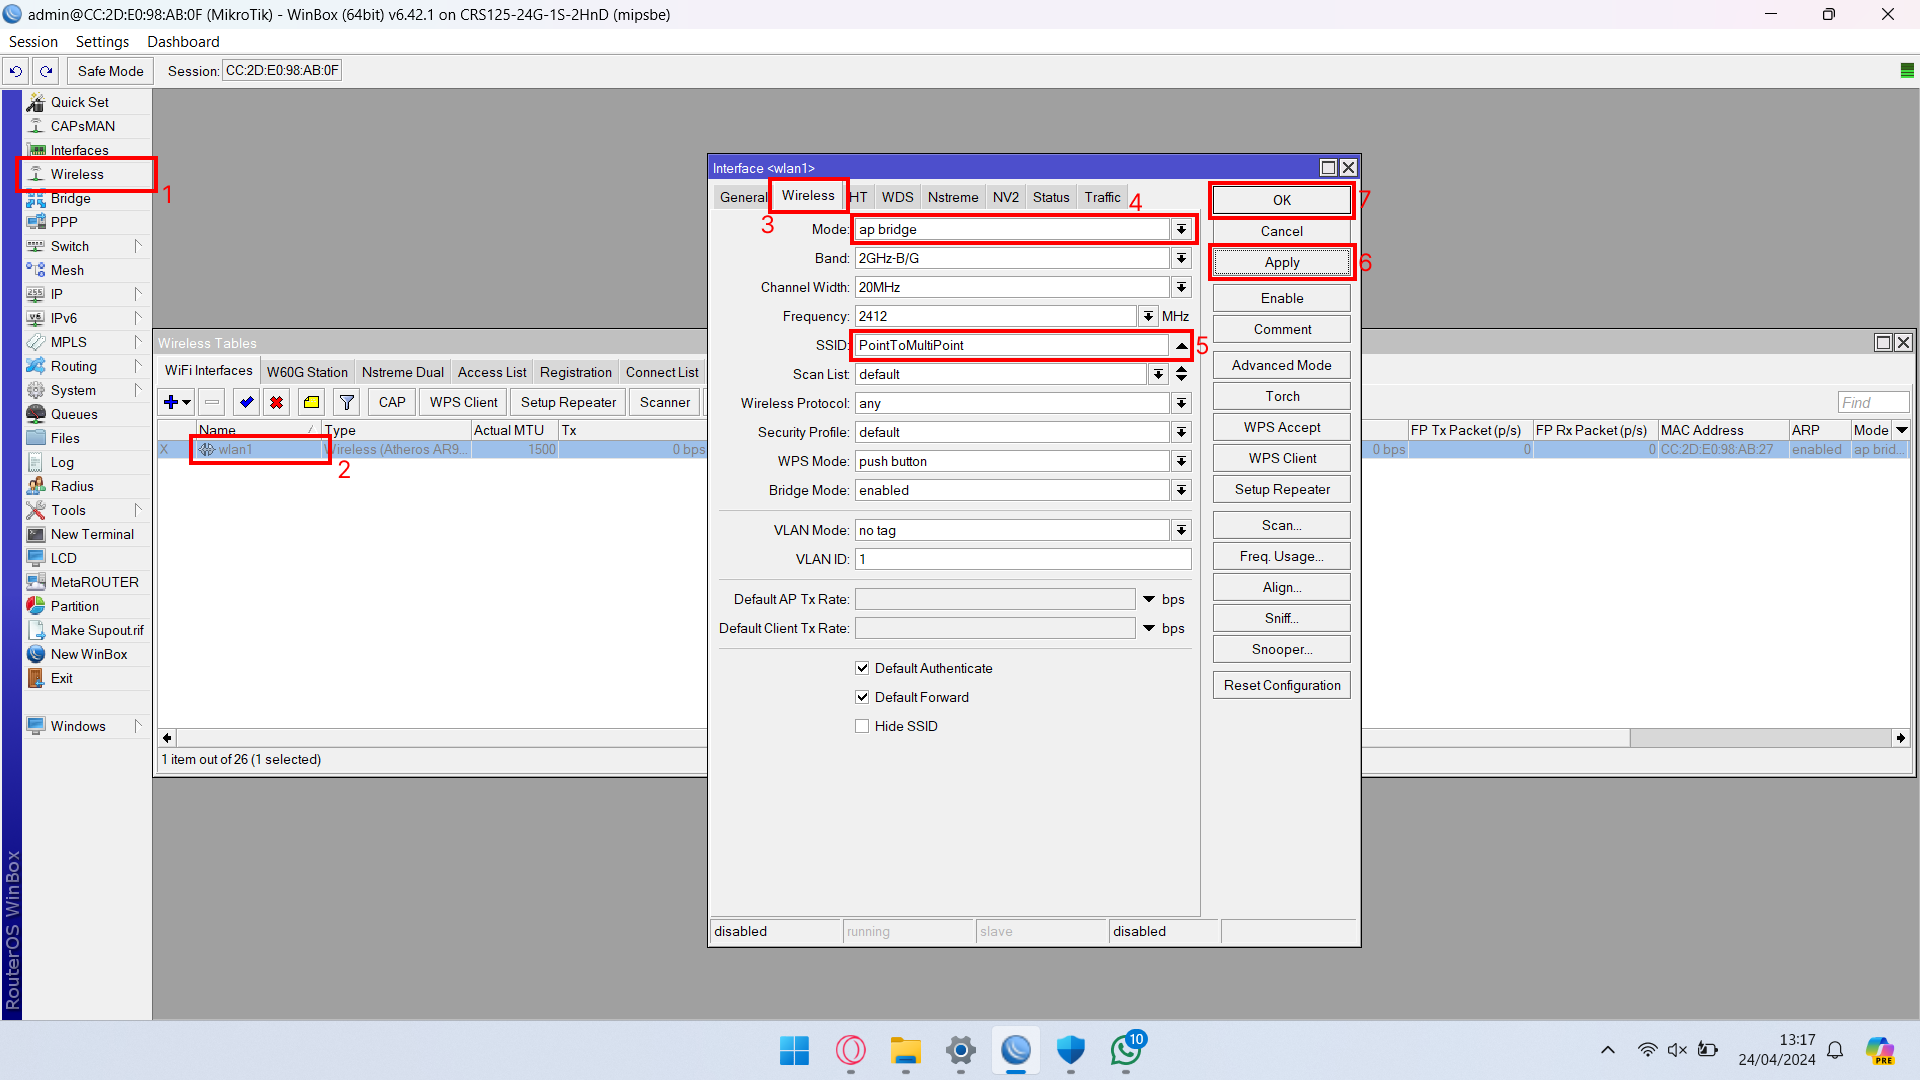
\includegraphics[width=0.9\linewidth]{P1/img/per2/pc1/Step 3.png}
			\caption{Step 2}
			\label{fig:Step 2(Per.2 PC1)}
		\end{figure}
	\end{enumerate}

	\textbf{Konfigurasi Router 2}
	\begin{enumerate}
		\item Berikan IP address pada interface wlan 1 yang dapat dibuat pada tab IP > Addresses. Berikan IP address sesuai dengan cara pengaturan IP address yang benar. Berikan IP address yang berbeda dengan contoh di modul.
		\begin{figure}[H]
			\centering
			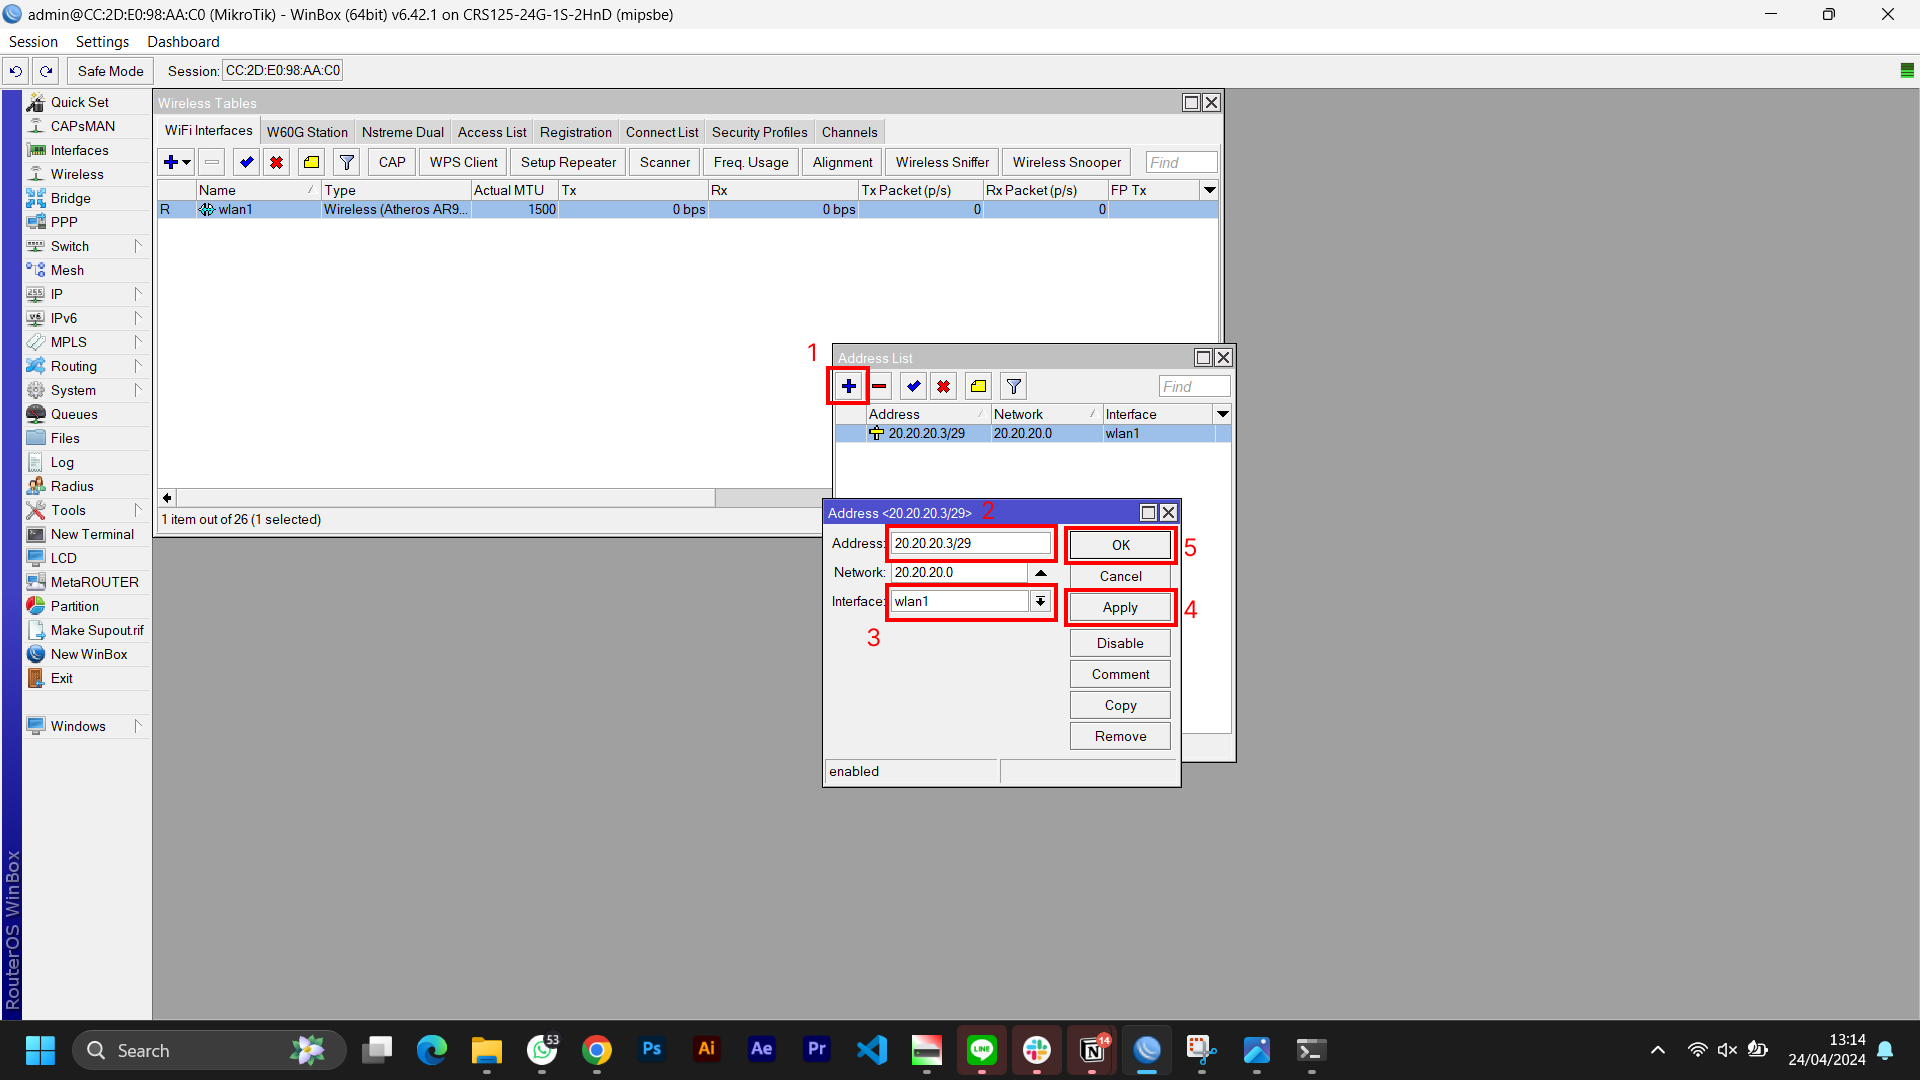
\includegraphics[width=0.9\linewidth]{P1/img/per1/pc2/Step 2.png}
			\caption{Step 1}
			\label{fig:Step 1(Per.2 PC2)}
		\end{figure}
		\item Atur Router 2 untuk mengaktifkan WLAN pada tab Wireless, pilih wlan1, lalu klik tombol centang. Kemudian atur WLAN pada mode station bridge. Kemudian cari sinyal yang sudah dipancarkan oleh Router 1, sesuai dengan nama SSID yang sudah dibuat
		\begin{figure}[H]
			\centering
			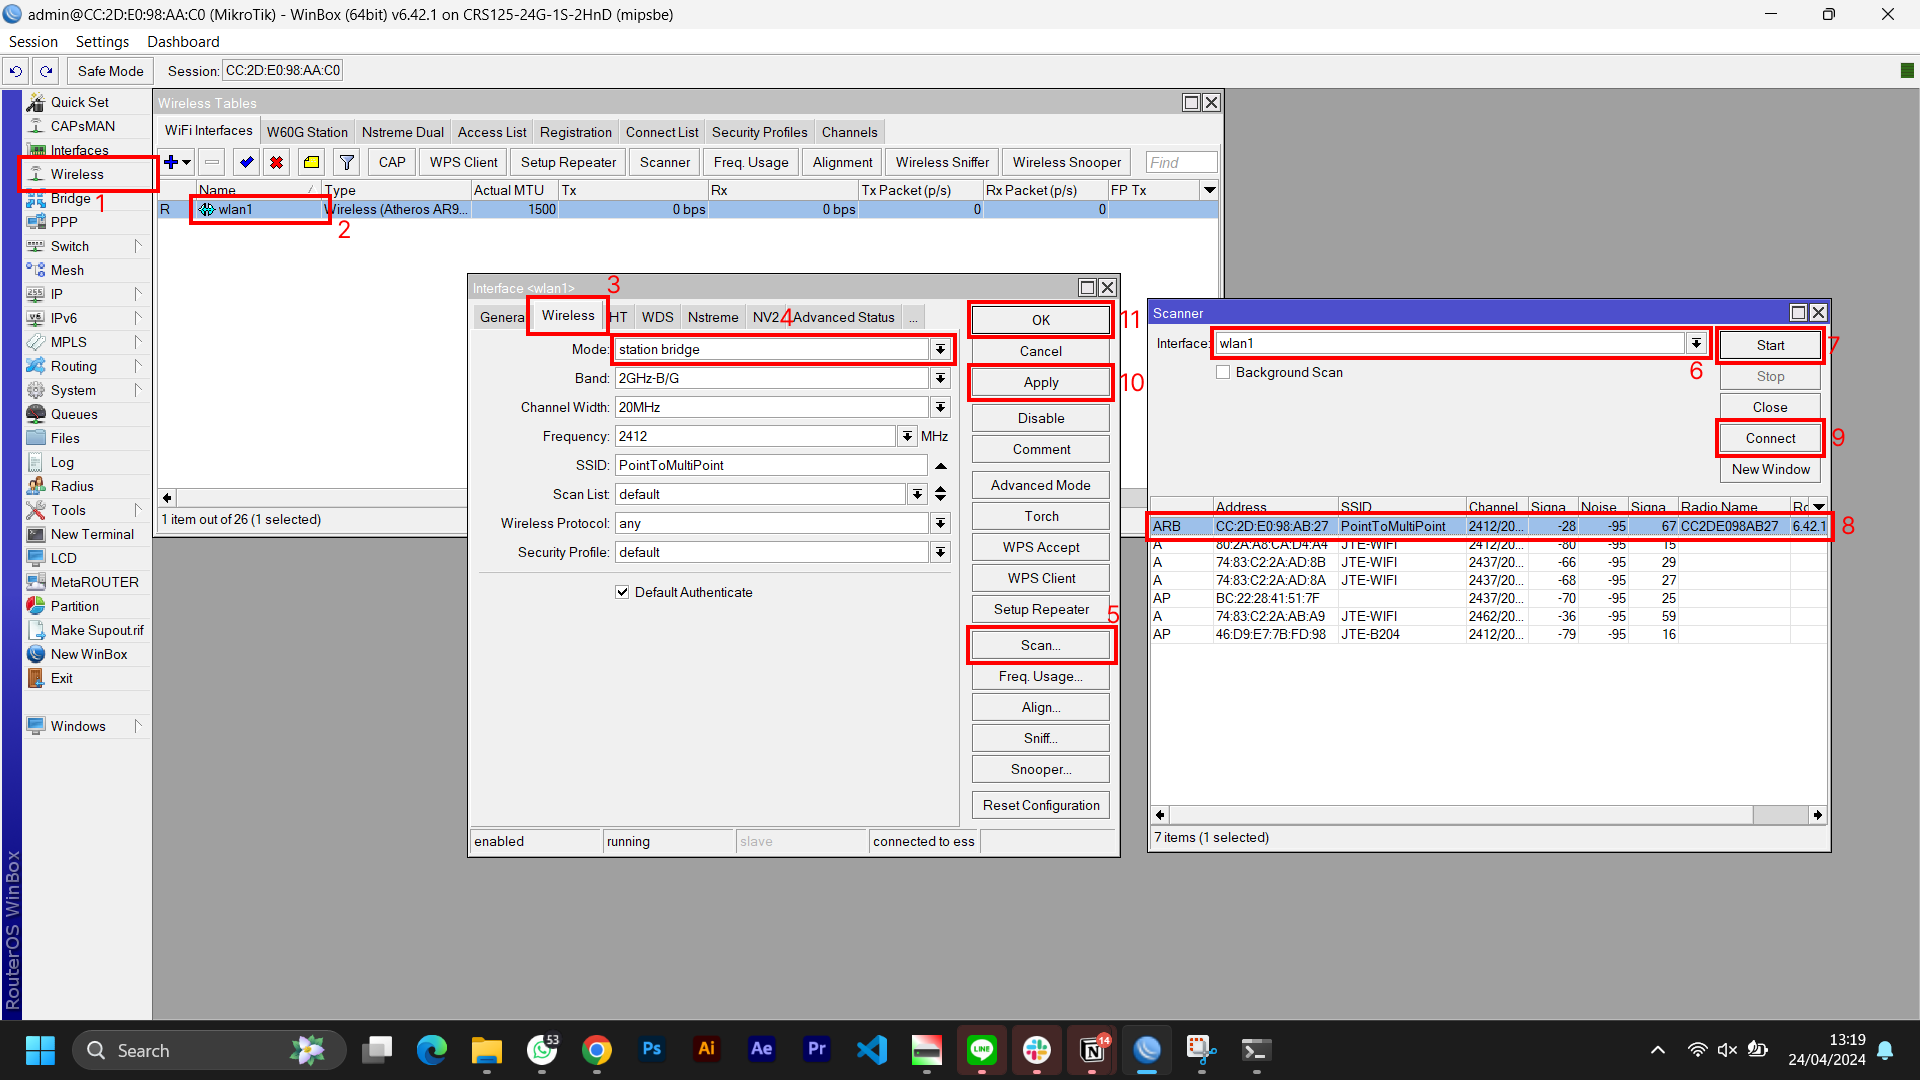
\includegraphics[width=0.9\linewidth]{P1/img/per2/pc2/Step 3.png}
			\caption{Step 2}
			\label{fig:Step 2(Per.2 PC2)}
		\end{figure}
	\end{enumerate}

	\textbf{Mengecek keberhasilan konfigurasi}
	\begin{enumerate}
		\item Lakukan test ping dari Router 1 ke Router 2
		\begin{figure}[H]
			\centering
			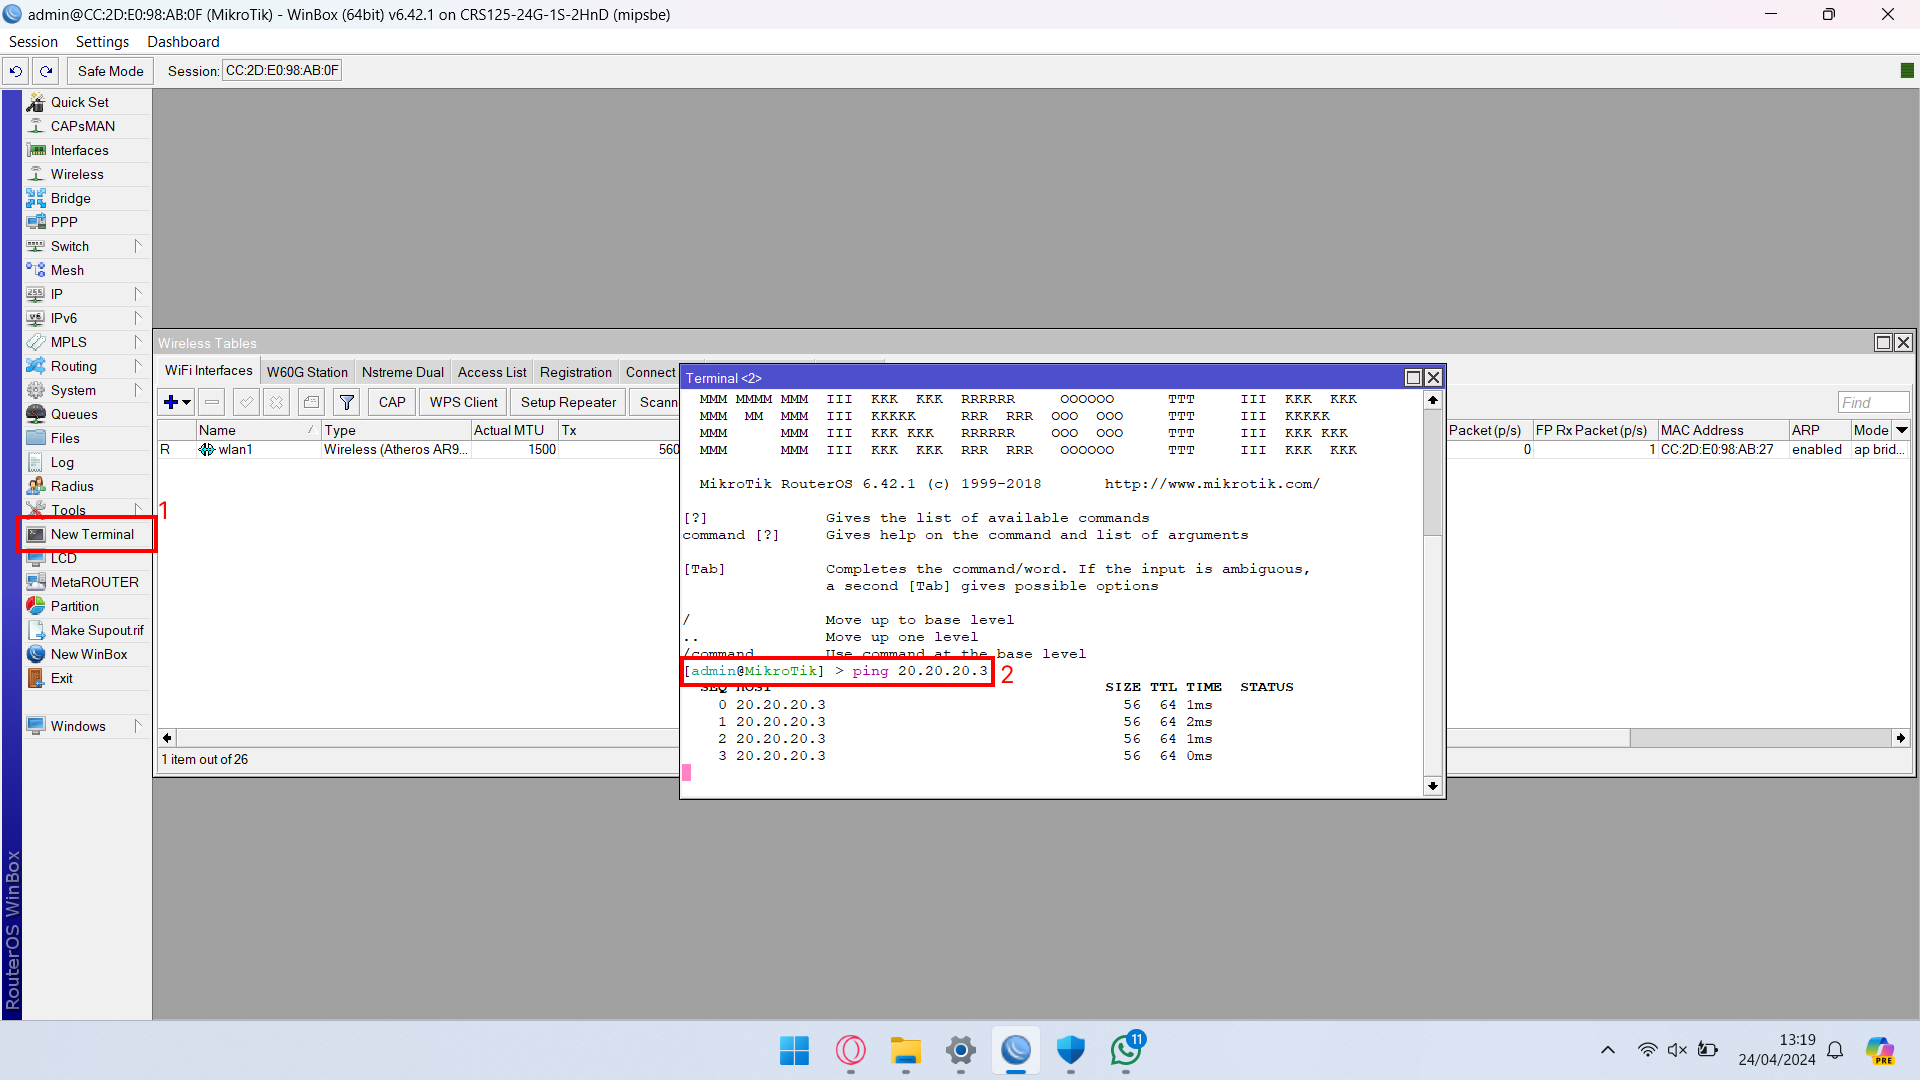
\includegraphics[width=0.9\linewidth]{P1/img/per2/pc1/Step 4.png}
			\caption{Step 1}
			\label{fig:Ping Step 1(Per.2 PC1)}
		\end{figure}
		\item Lakukan test ping dari Router 2 ke Router 1
		\begin{figure}[H]
			\centering
			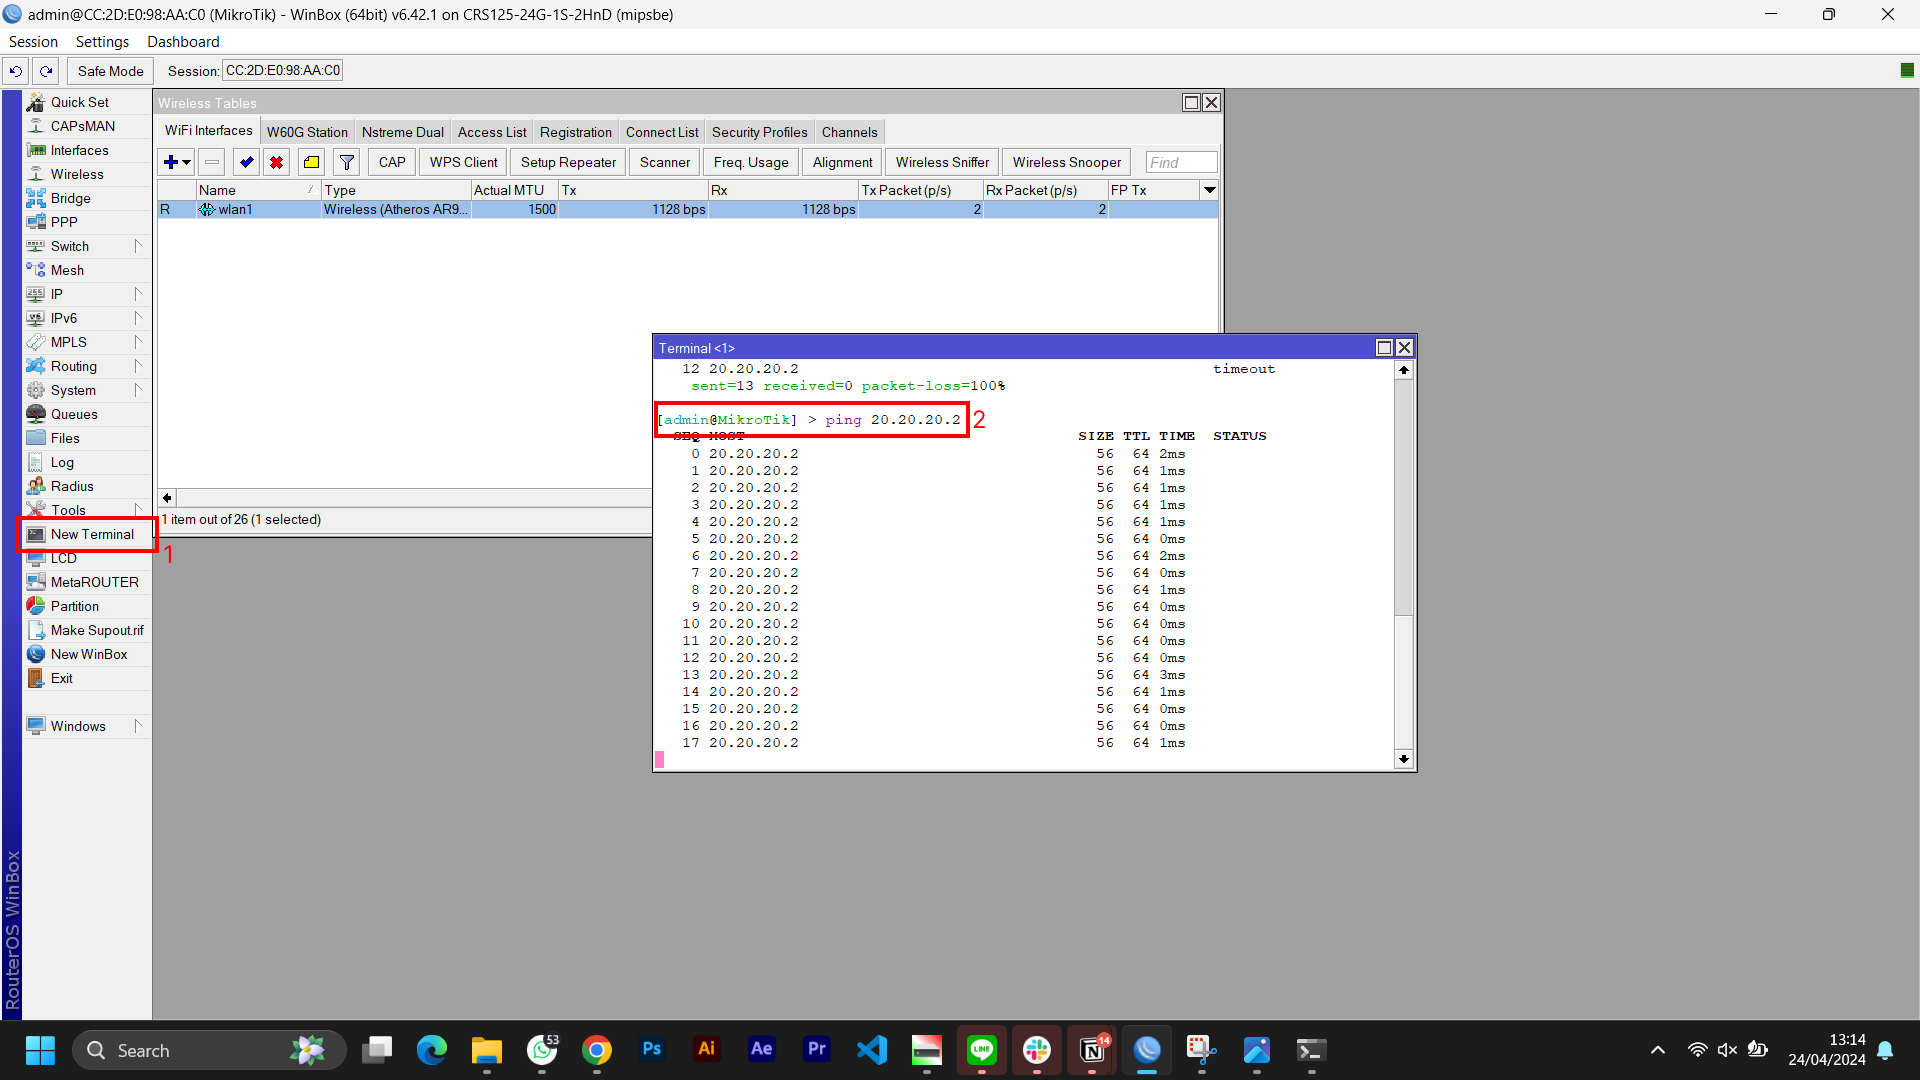
\includegraphics[width=0.9\linewidth]{P1/img/per1/pc2/Step 4.png}
			\caption{Step 1}
			\label{fig:Ping Step 2(Per.2 PC2)}
		\end{figure}
	\end{enumerate}
\end{center}

%======================PERCOBAAN 3==========================%
\subsection{Wireless Bridge}
Untuk wireless bridge ini sangatlah sederhana, koneksi ini sangat jarang ditemui pada
implementasi realnya, konfigurasi ini menjadikan seolah-olah koneksi yang terhubung
menggunakan switch, keunggulan yang saya rasakan yaitu ringannya kinerja router yang
menggunakan koneksi ini. Untuk konfigurasinya seperti berikut.
Untuk gambar topologi sama dengan Point To Point, hanya saja berbeda di konfigurasi dan
mode pada routernya.
\begin{center}
	\textbf{Konfigurasi Router 1}
	\begin{enumerate}
		\item Buka WinBox dan lakukan koneksi ke Router
		\item Berikan IP address pada interface wlan1 dan ethernet 2 yang dapat dibuat pada tab IP > Addresses. Berikan IP address sesuai dengan cara pengaturan IP address yang benar. Berikan IP address yang berbeda dengan contoh di modul.
		\begin{figure}[H]
			\centering
			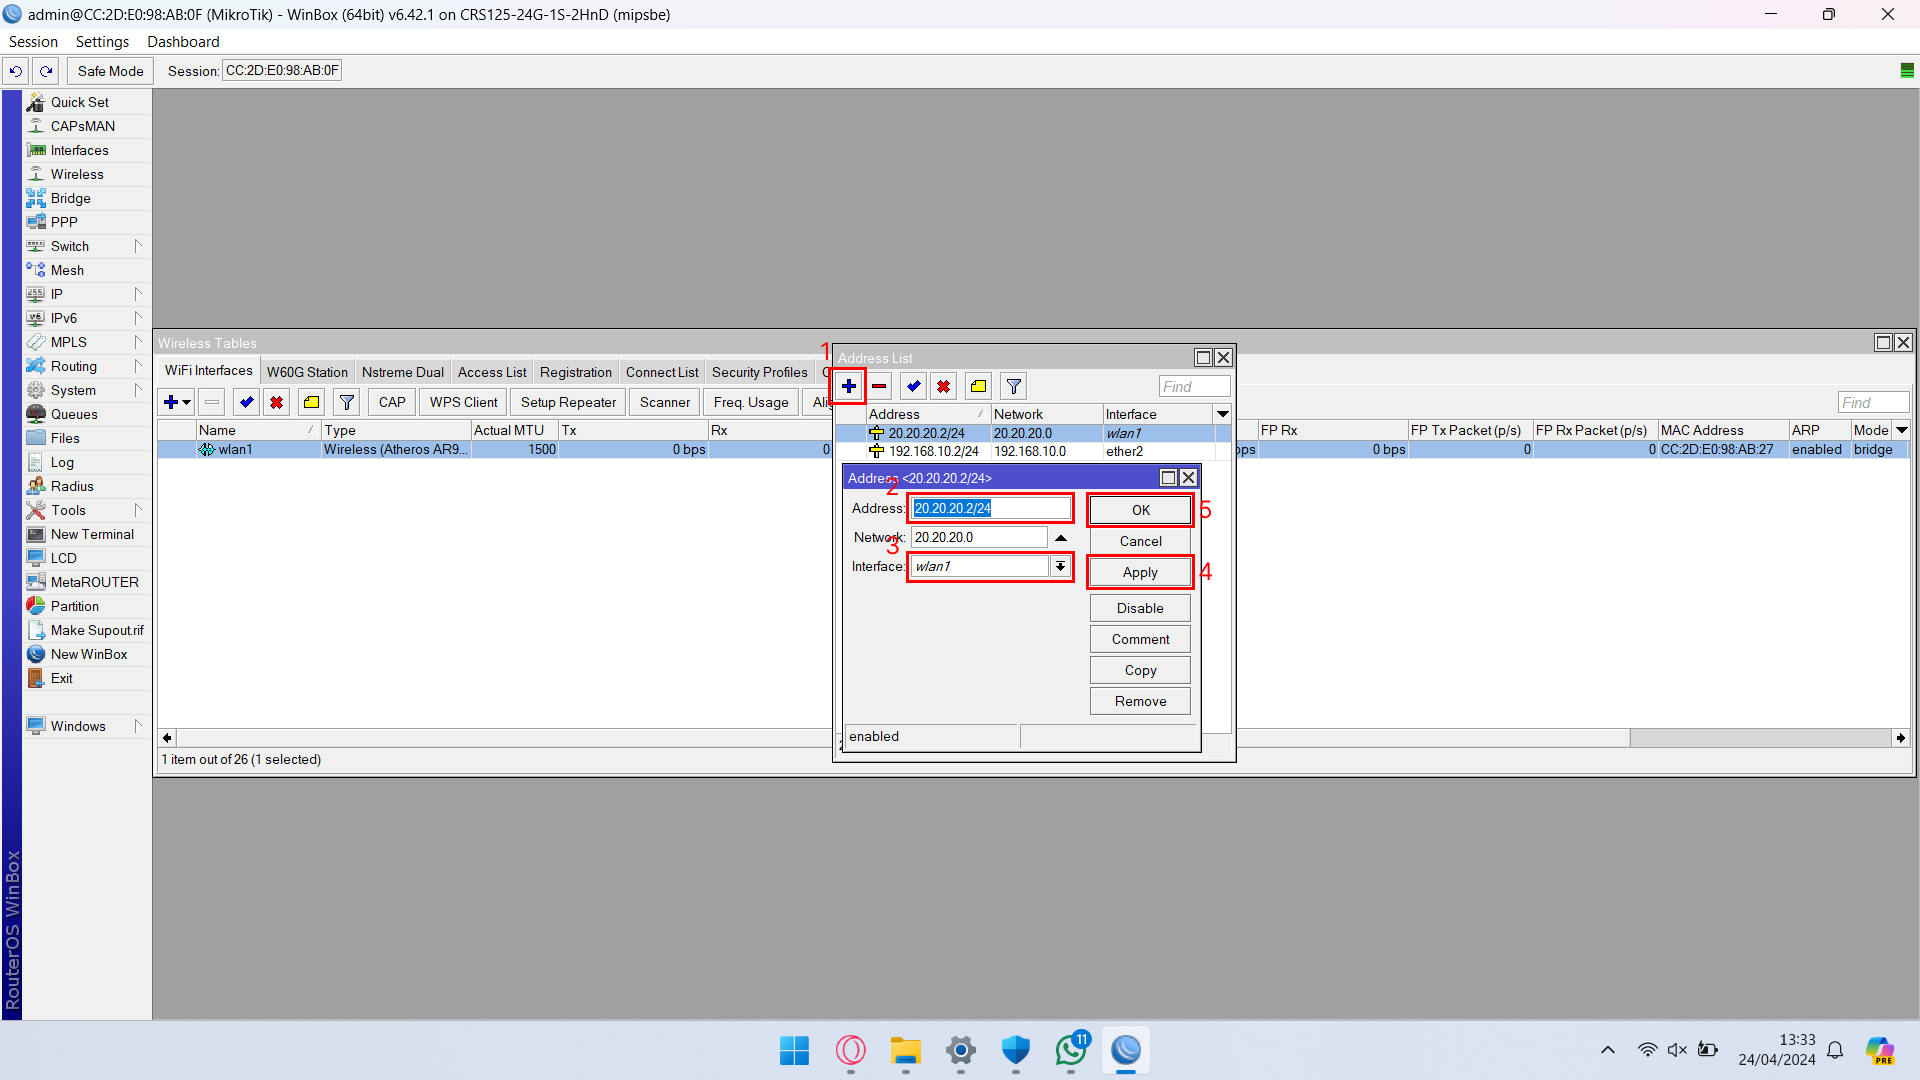
\includegraphics[width=0.9\linewidth]{P1/img/per3/pc1/Step 2.png}
			\caption{Step 2}
			\label{fig:Step 2(Per.3 PC1)}
		\end{figure}
		\item Atur Router 1 untuk mengaktifkan WLAN pada tab Wireless, pilih wlan1, lalu klik tombol centang. Kemudian atur WLAN pada mode bridge dan isi SSID yang diinginkan. Berikan SSID sekreatif mungkin, yang berbeda dengan contoh di modul.
		\begin{figure}[H]
			\centering
			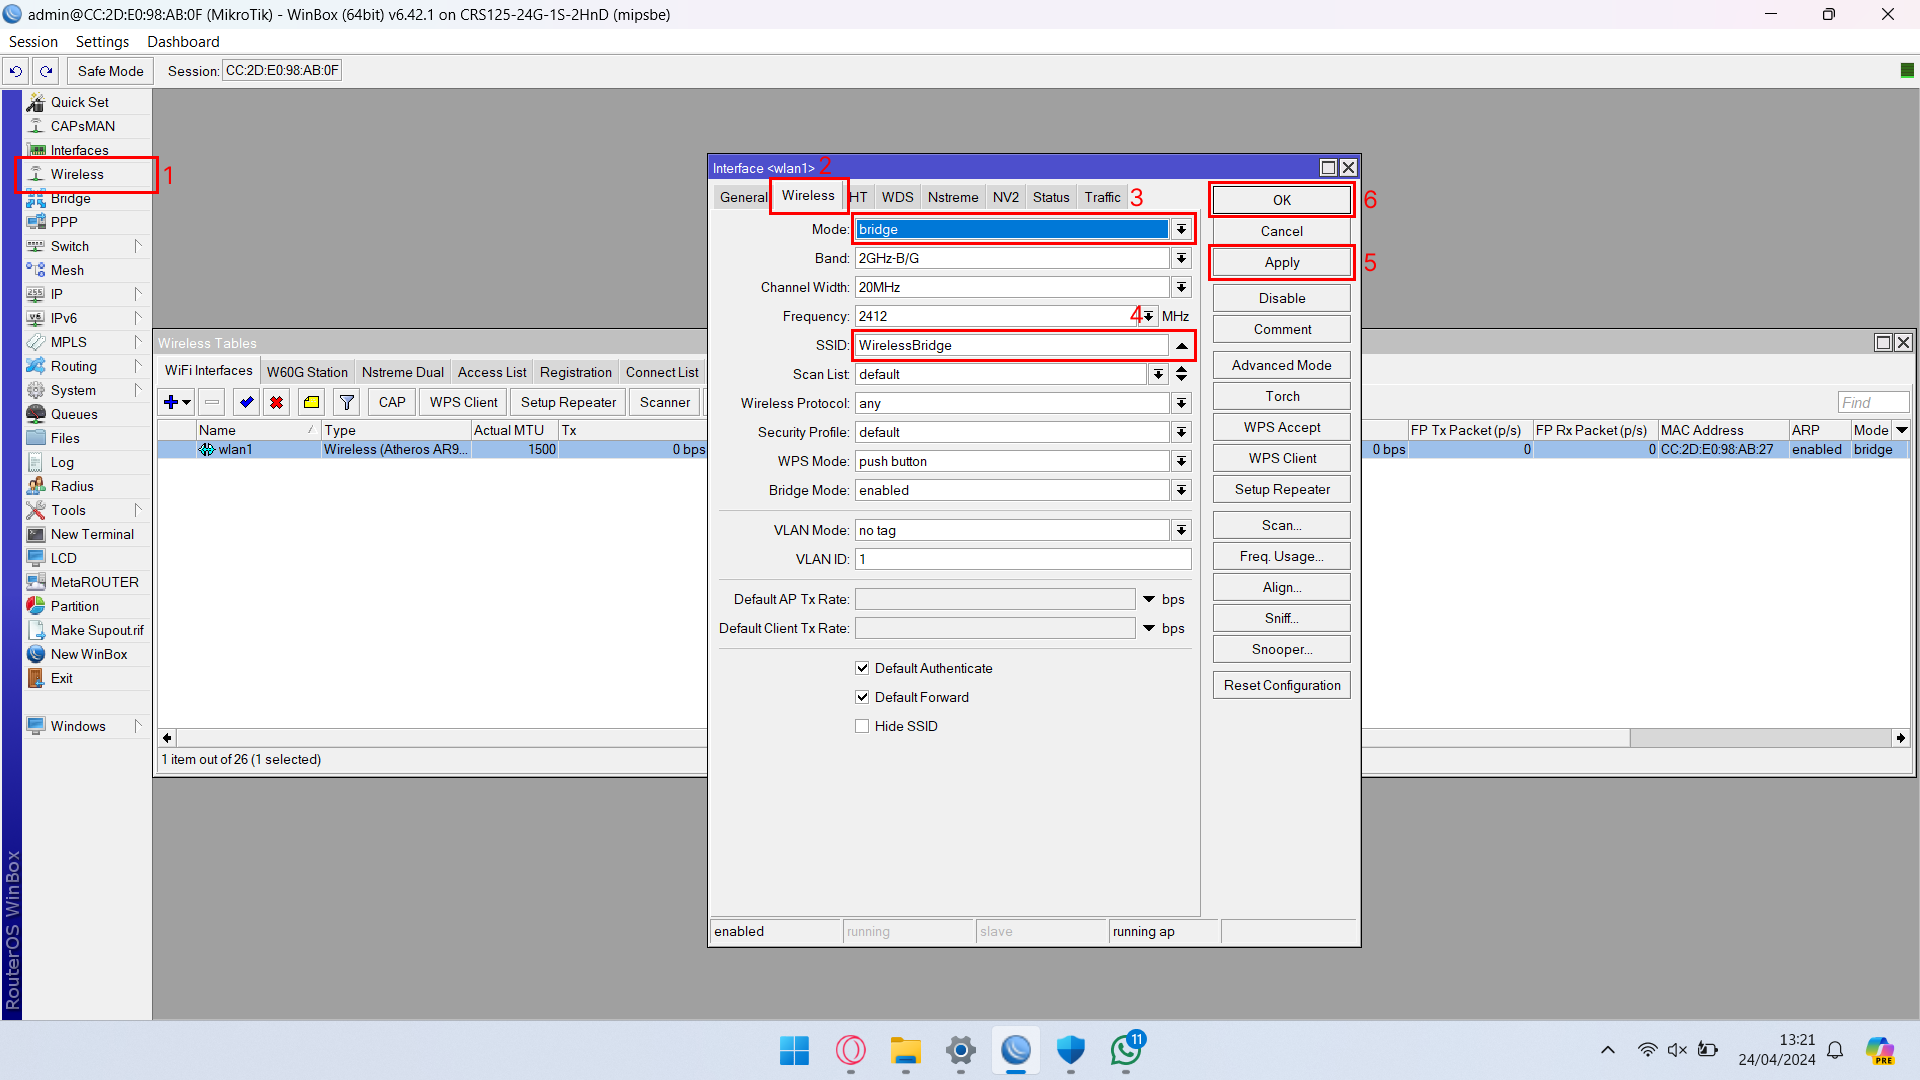
\includegraphics[width=0.9\linewidth]{P1/img/per3/pc1/Step 3.png}
			\caption{Step 3}
			\label{fig:Step 3(Per.3 PC1)}
		\end{figure}
		\item Tambahkan bridge pada Router 1 untuk menghubungkan interface wlan1 dan ether 2. Buat bridge pada tab Bridge dan beri nama yang diinginkan.
		\begin{figure}[H]
			\centering
			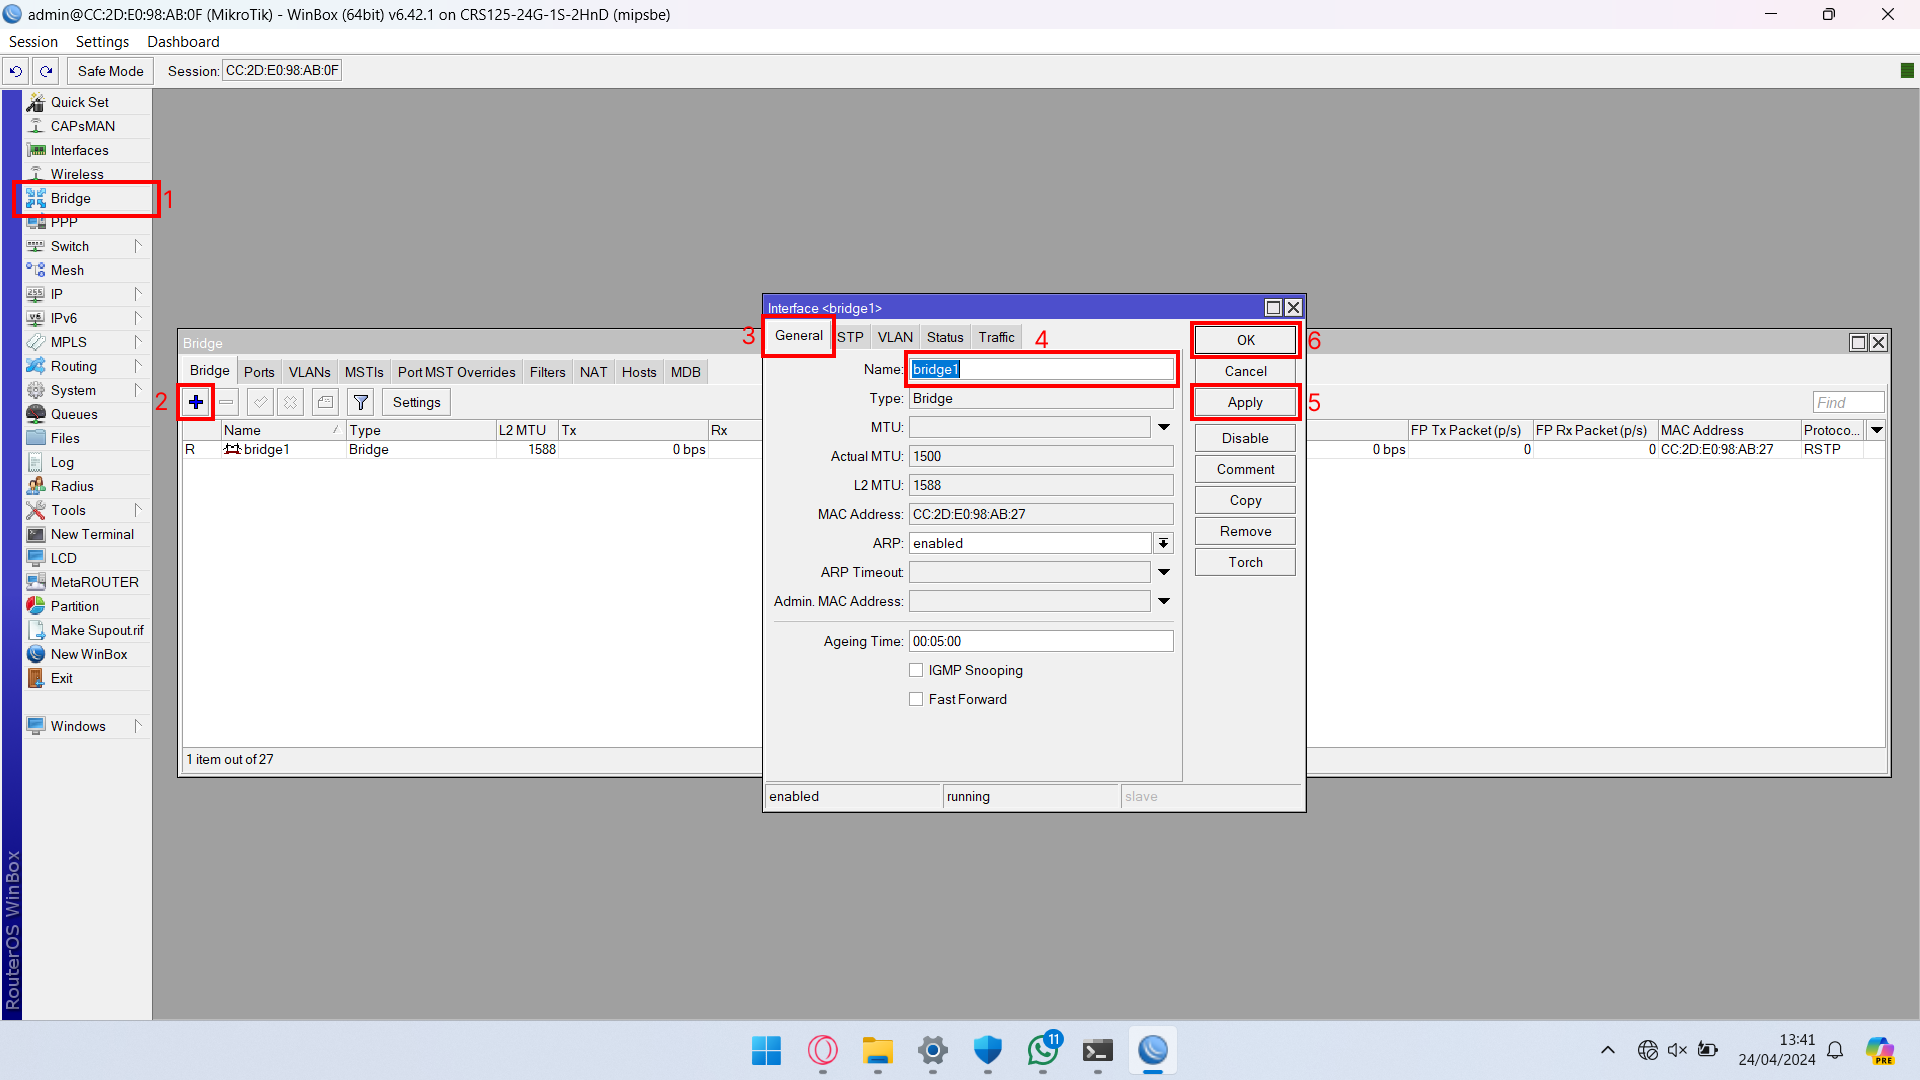
\includegraphics[width=0.9\linewidth]{P1/img/per3/pc1/Step 4.png}
			\caption{Step 4}
			\label{fig:Step 4(Per.3 PC1)}
		\end{figure}
		\item Selanjutnya tambahkan port interface yang akan dihubungkan pada tab Ports, dan tambahkan interface wlan1 dan ehter2 pada bridge sesuai yang telah dibuat sebelumnya.
		\begin{figure}[H]
			\centering
			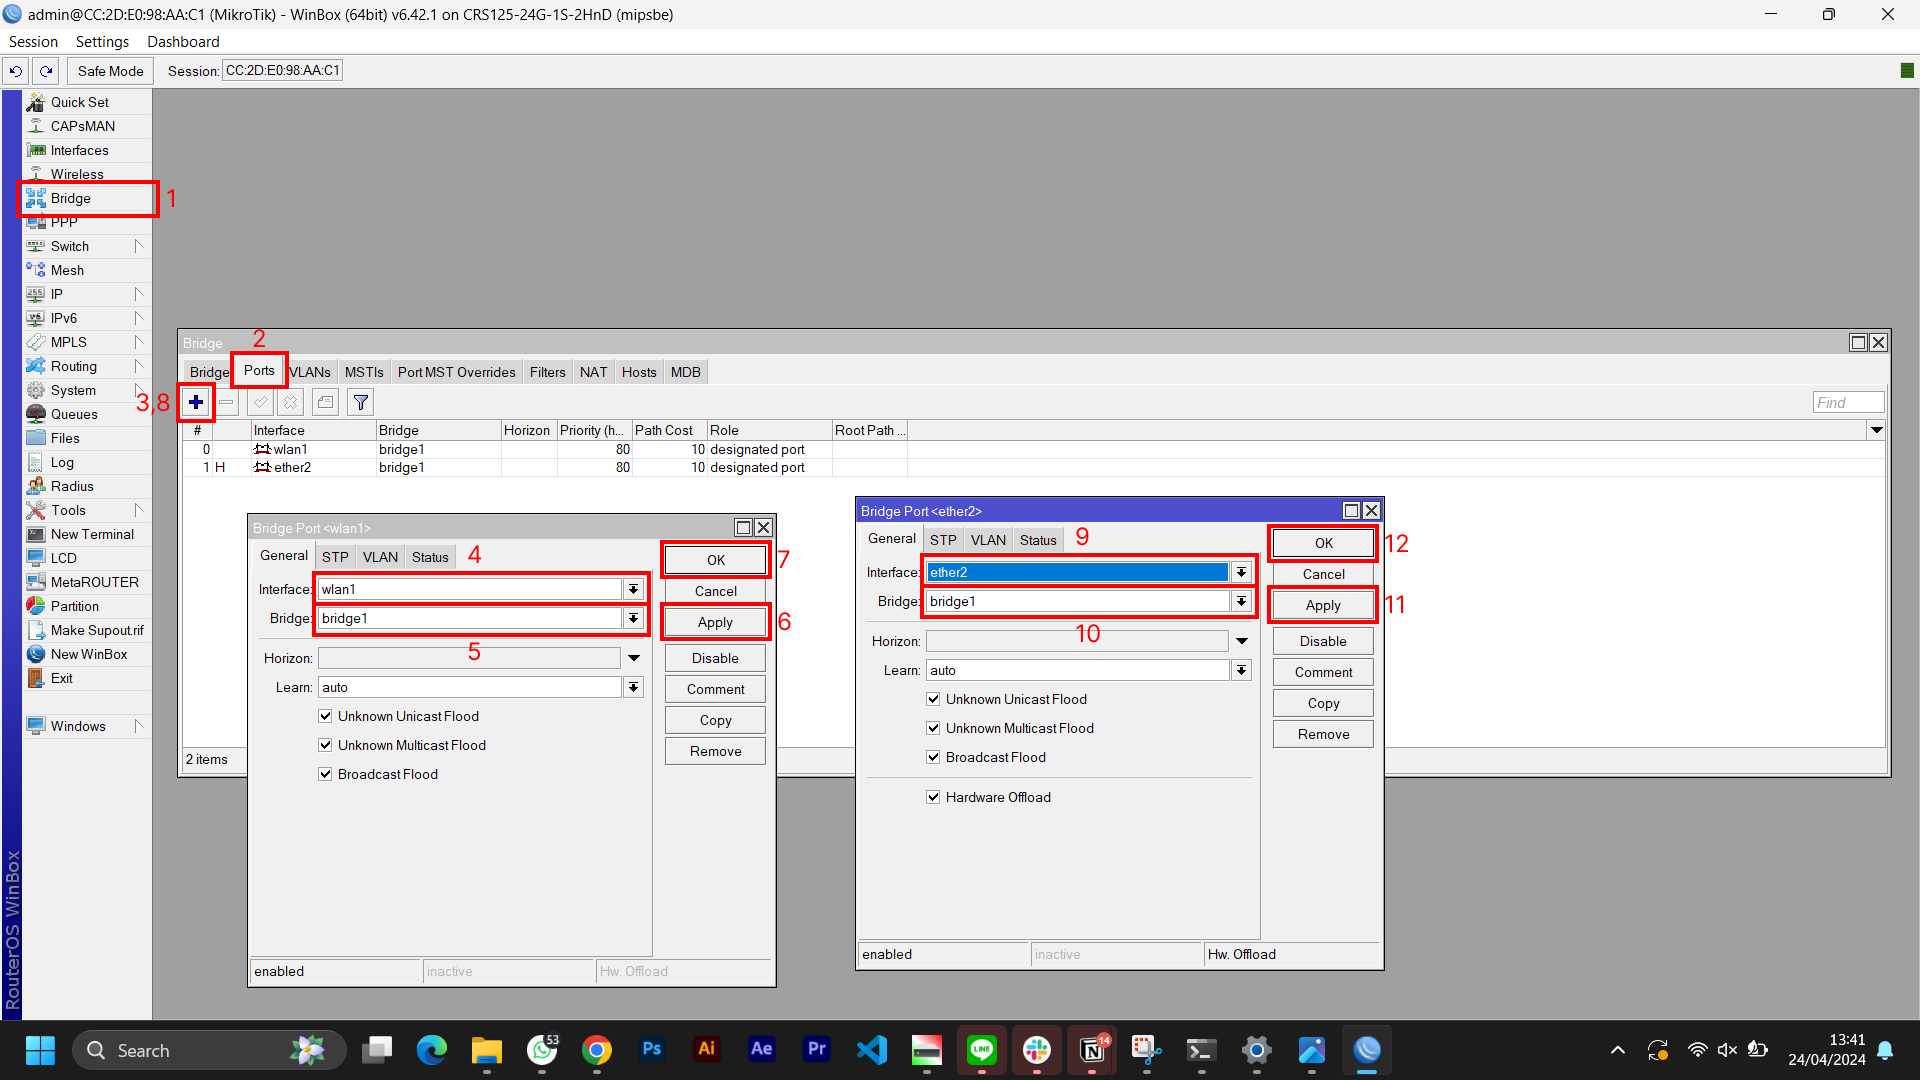
\includegraphics[width=0.9\linewidth]{P1/img/per3/pc1/Step 5.png}
			\caption{Step 5}
			\label{fig:Step 5(Per.3 PC1)}
		\end{figure}
		\item Atur IP pada PC 1 dengan mengubah pengaturan pada setting ethernet. Ubah IP perangkat yang otomatis menjadi manual, pastikan IP PC 1 masih satu jaringan dengan IP lokal yang diinginkan, isi Gateway dengan IP Router yang tersambung dengan PC. Berikan IP address yang berbeda dengan contoh yang ada di modul.
		\begin{figure}[H]
			\centering
			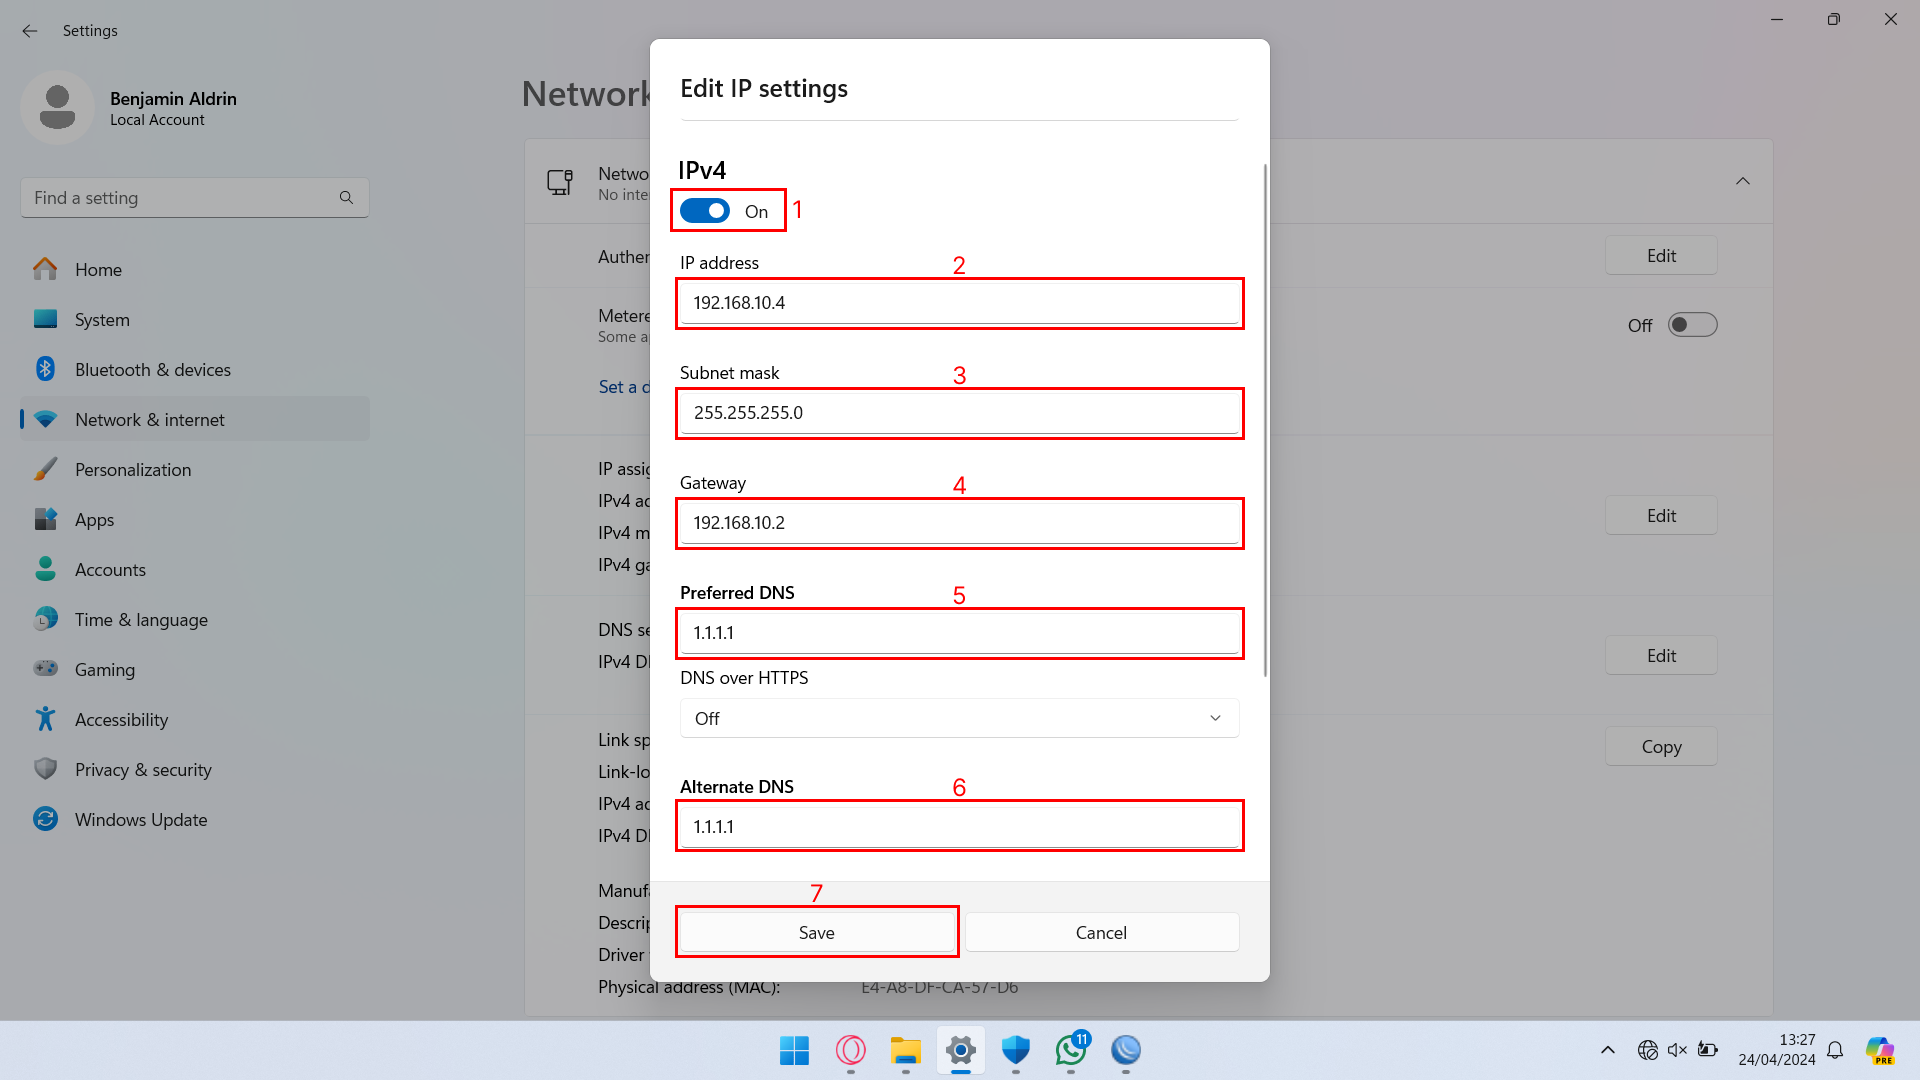
\includegraphics[width=0.9\linewidth]{P1/img/per3/pc1/Step 6.png}
			\caption{Step 6}
			\label{fig:Step 6(Per.3 PC1)}
		\end{figure}
	\end{enumerate}

	\textbf{Konfigurasi Router 2}
	\begin{enumerate}
		\item Buka WinBox dan lakukan koneksi ke Router
		\item Berikan IP address pada interface wlan1 dan ethernet 2 yang dapat dibuat pada tab IP > Addresses. Berikan IP address sesuai dengan cara pengaturan IP address yang benar. Berikan IP address yang berbeda dengan contoh di modul.
		\begin{figure}[H]
			\centering
			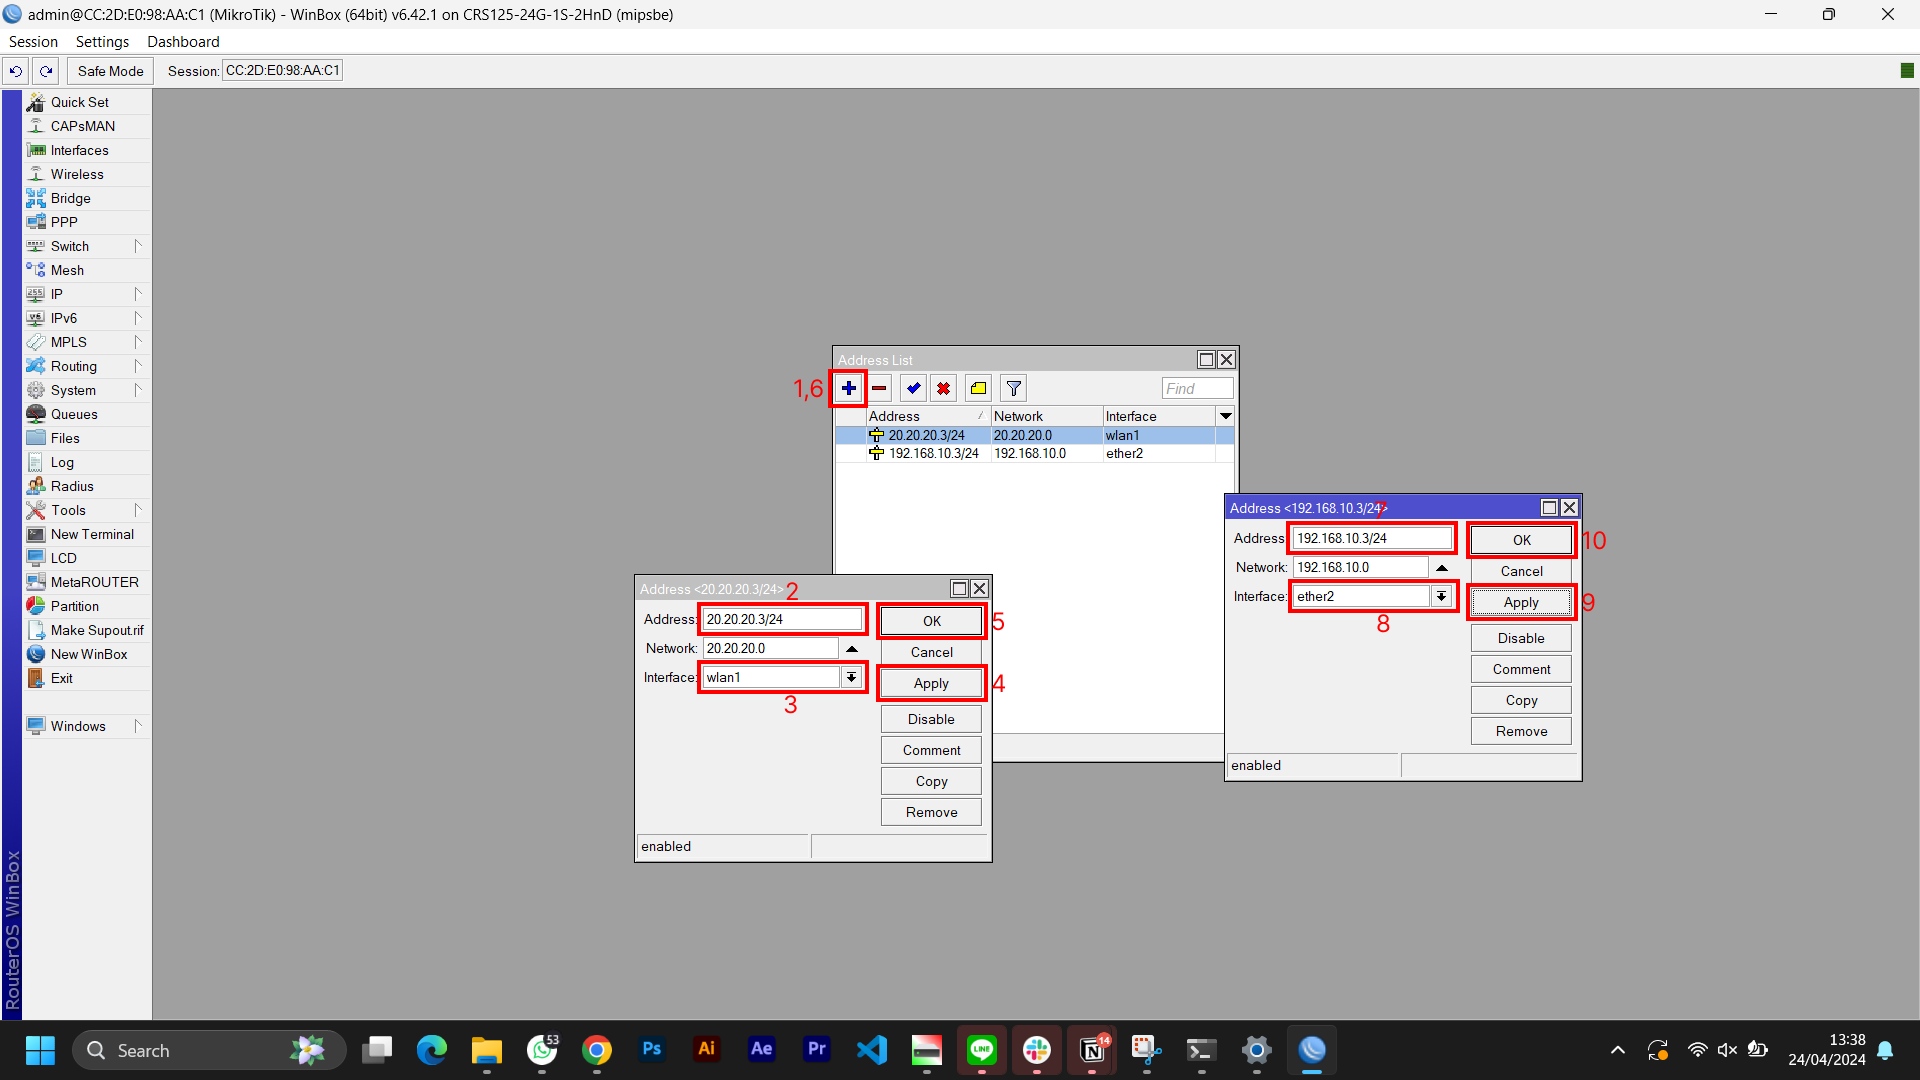
\includegraphics[width=0.9\linewidth]{P1/img/per3/pc2/Step 2.png}
			\caption{Step 2}
			\label{fig:Step 2(Per.3 PC2)}
		\end{figure}
		\item Atur Router 2 untuk mengaktifkan WLAN pada tab Wireless, pilih wlan1, lalu klik tombol centang. Kemudian atur WLAN pada mode station pseudobridge. Kemudian cari sinyal yang sudah dipancarkan oleh Router 1, sesuai dengan nama SSID yang sudah dibuat.
		\begin{figure}[H]
			\centering
			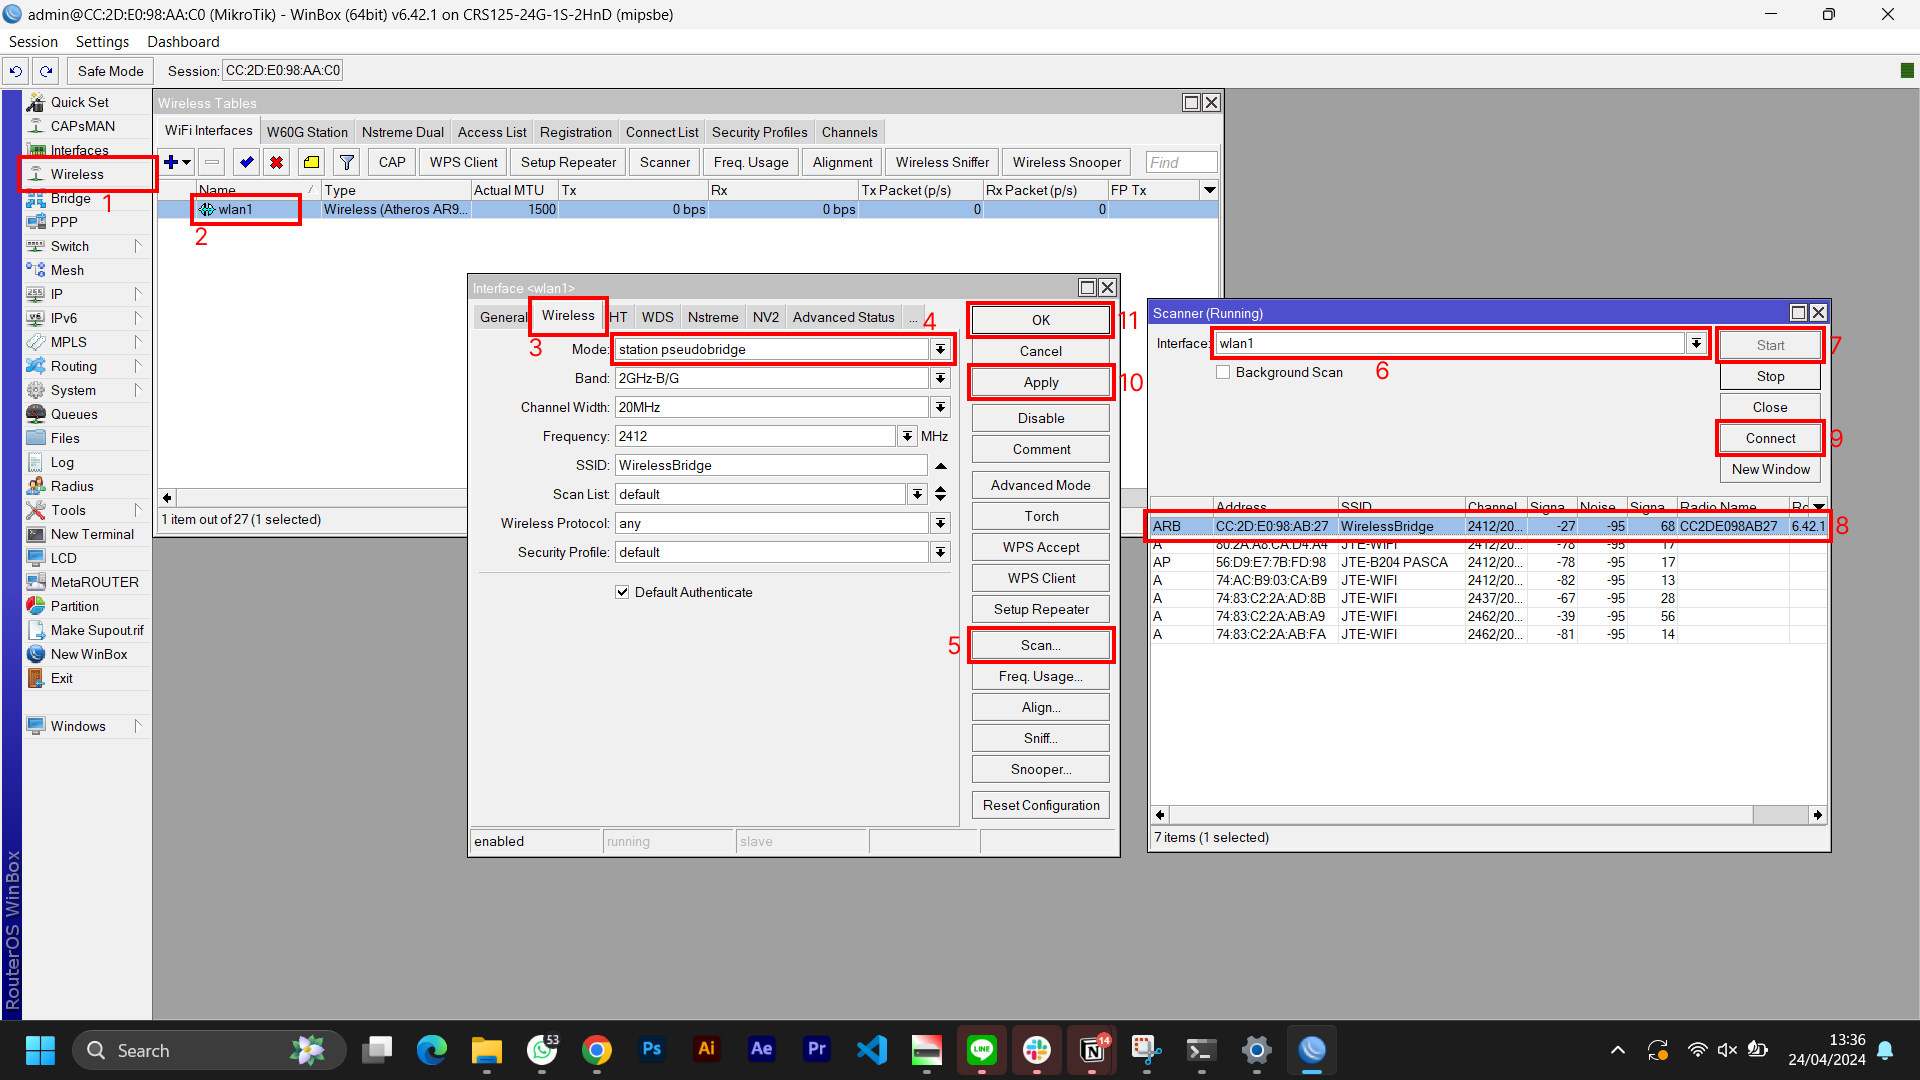
\includegraphics[width=0.9\linewidth]{P1/img/per3/pc2/Step 3.png}
			\caption{Step 3}
			\label{fig:Step 3(Per.3 PC2)}
		\end{figure}
		\item Tambahkan bridge pada Router 2 untuk menghubungkan interface wlan1 dan ether 2. Buat bridge pada tab Bridge dan beri nama yang diinginkan.
		\begin{figure}[H]
			\centering
			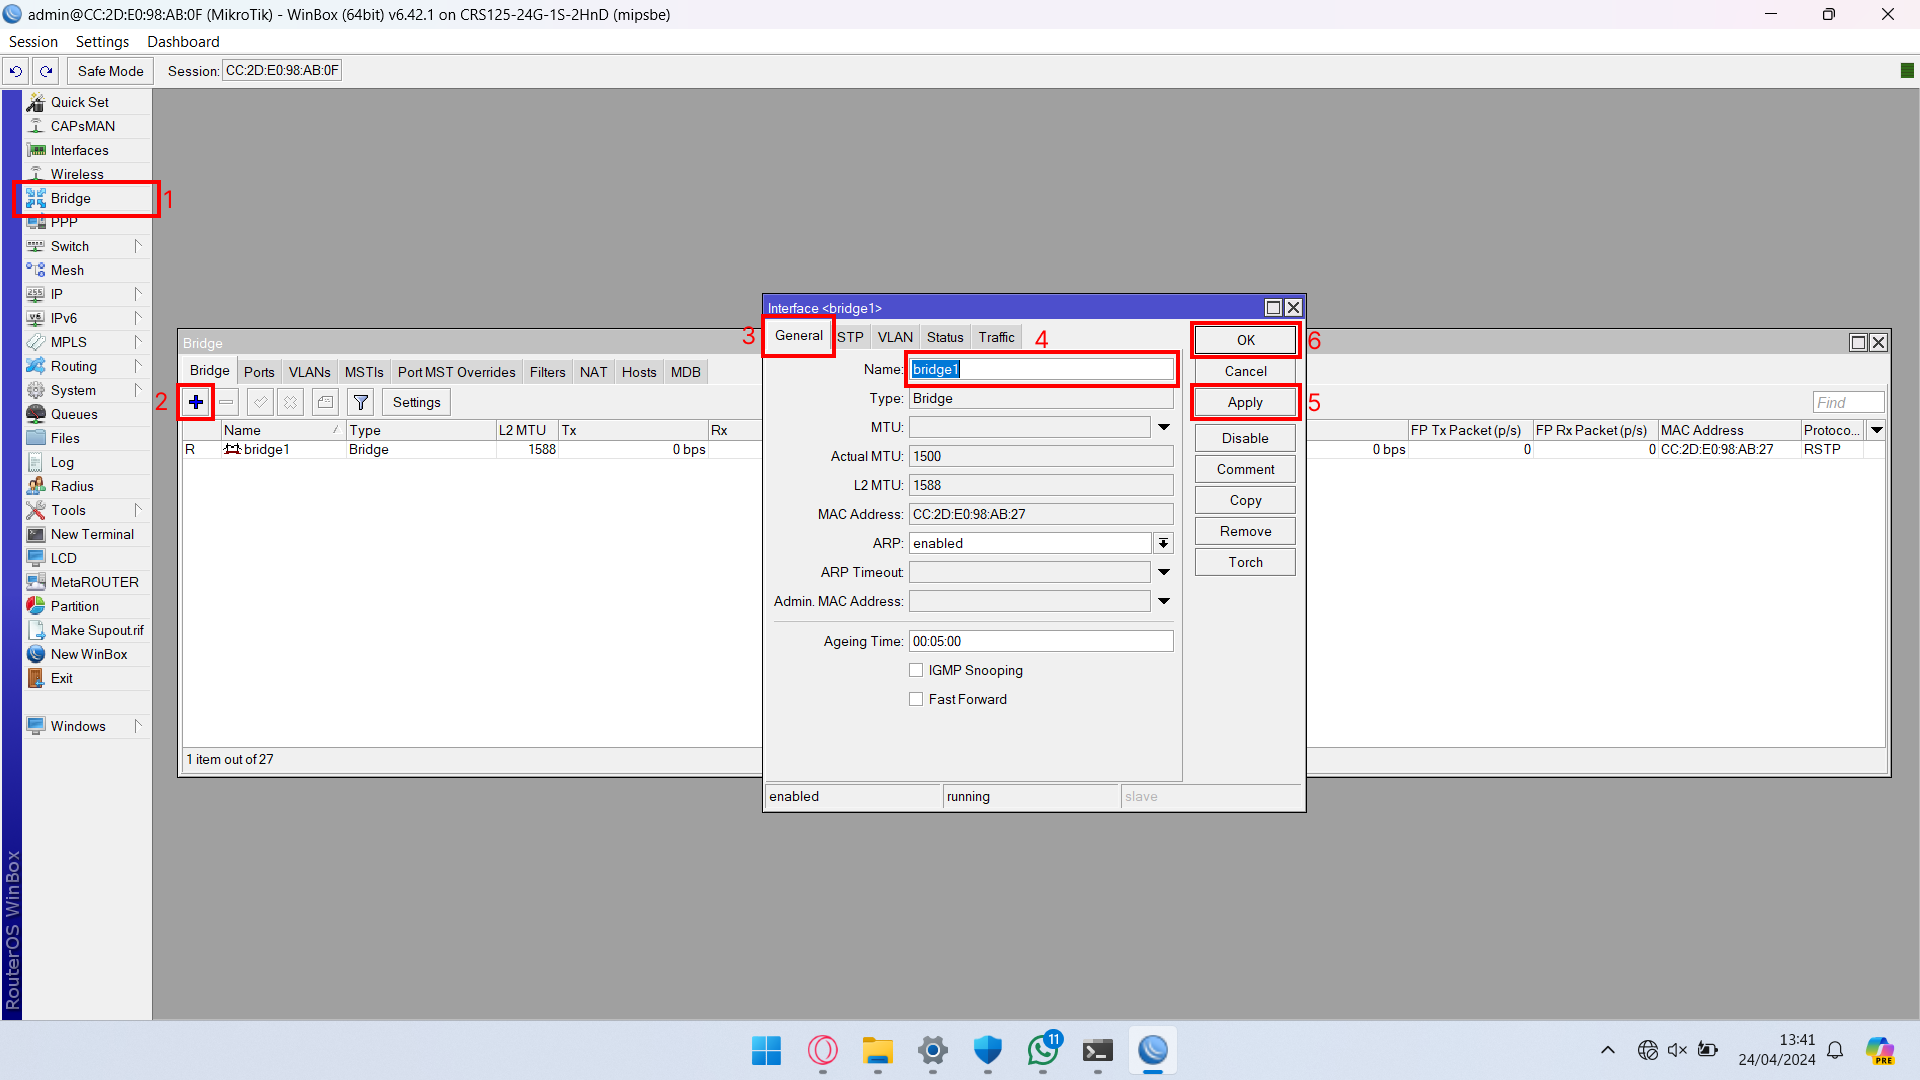
\includegraphics[width=0.9\linewidth]{P1/img/per3/pc1/Step 4.png}
			\caption{Step 4}
			\label{fig:Step 4(Per.3 PC2)}
		\end{figure}
		\item Selanjutnya tambahkan port interface yang akan dihubungkan pada tab Ports, dan tambahkan interface wlan1 dan ehter2 pada bridge sesuai yang telah dibuat sebelumnya.
		\begin{figure}[H]
			\centering
			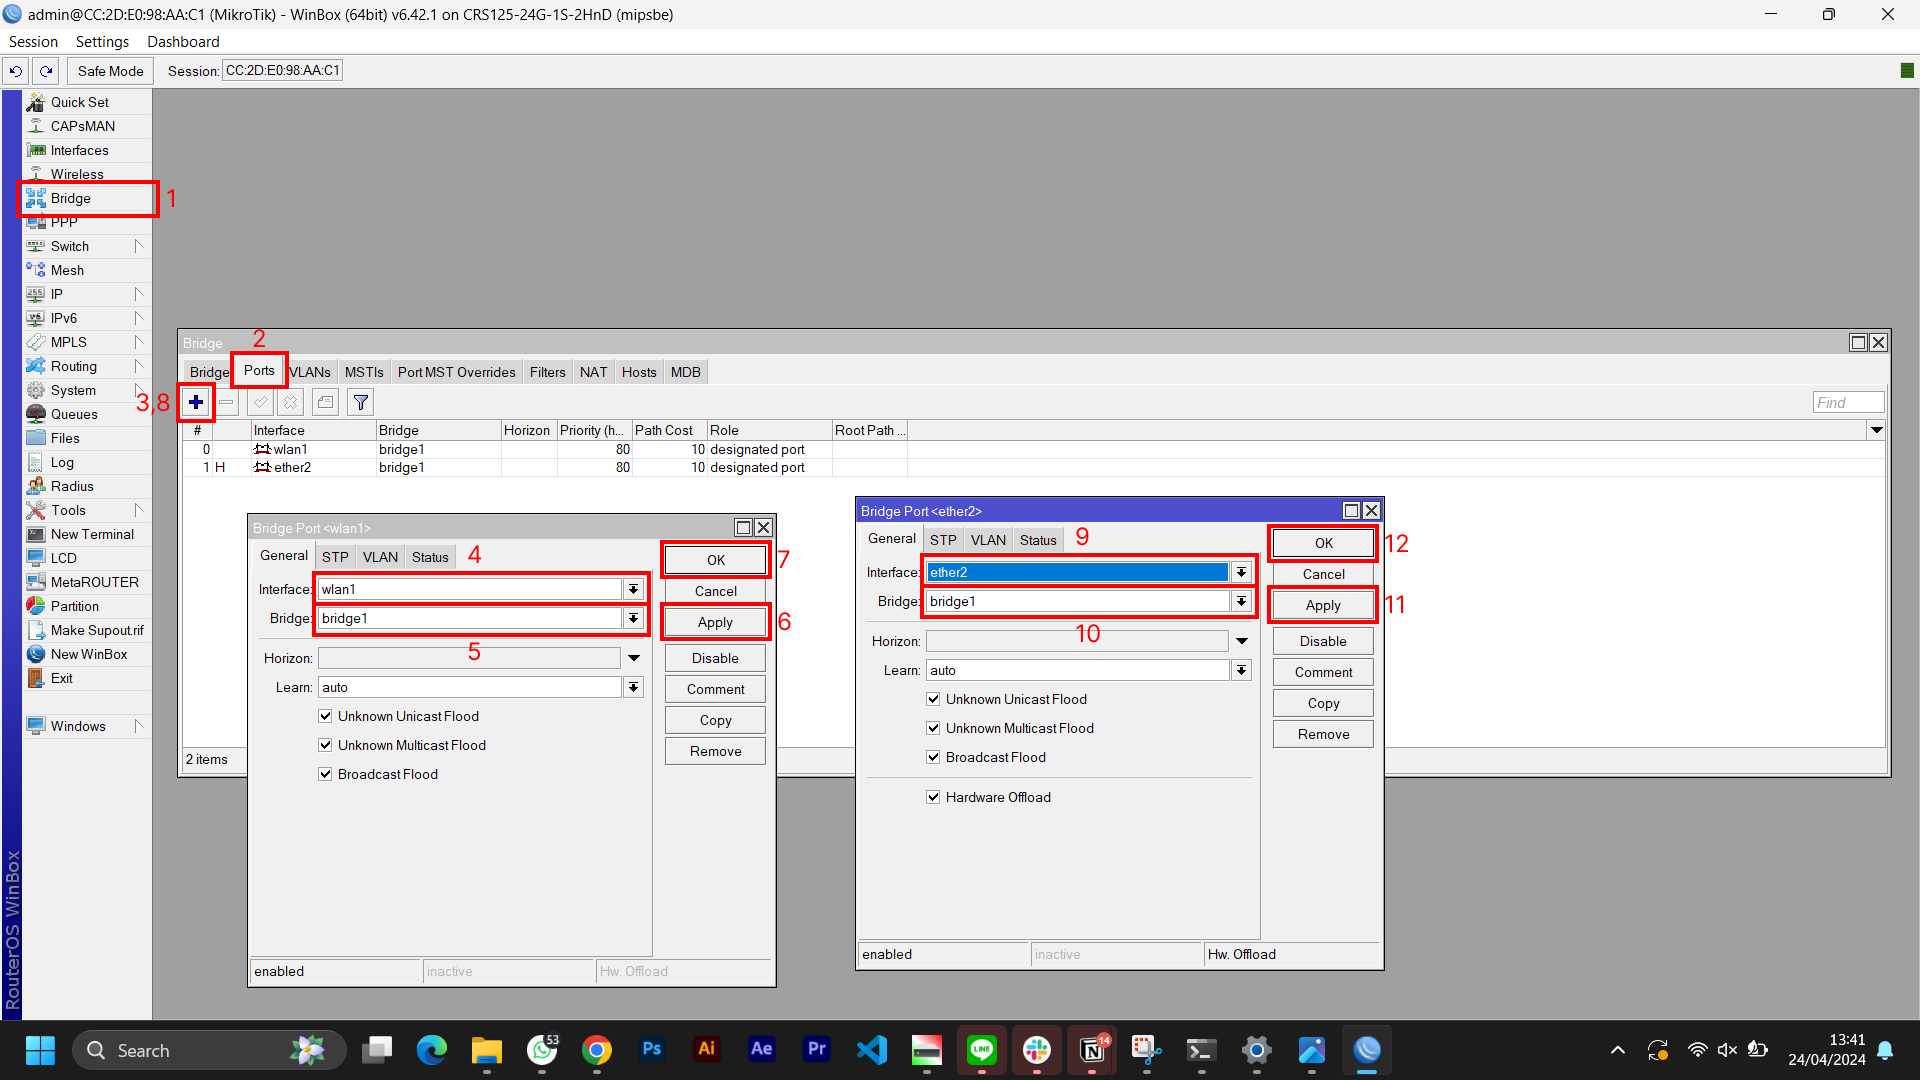
\includegraphics[width=0.9\linewidth]{P1/img/per3/pc1/Step 5.png}
			\caption{Step 5}
			\label{fig:Step 5(Per.3 PC2)}
		\end{figure}
		\item Atur IP pada PC 2 dengan mengubah pengaturan pada setting ethernet. Ubah IP perangkat yang otomatis menjadi manual, pastikan IP PC 2 masih satu jaringan dengan IP lokal yang diinginkan, isi Gateway dengan IP Router yang tersambung dengan PC. Berikan IP address yang berbeda dengan contoh yang ada di modul.
		\begin{figure}[H]
			\centering
			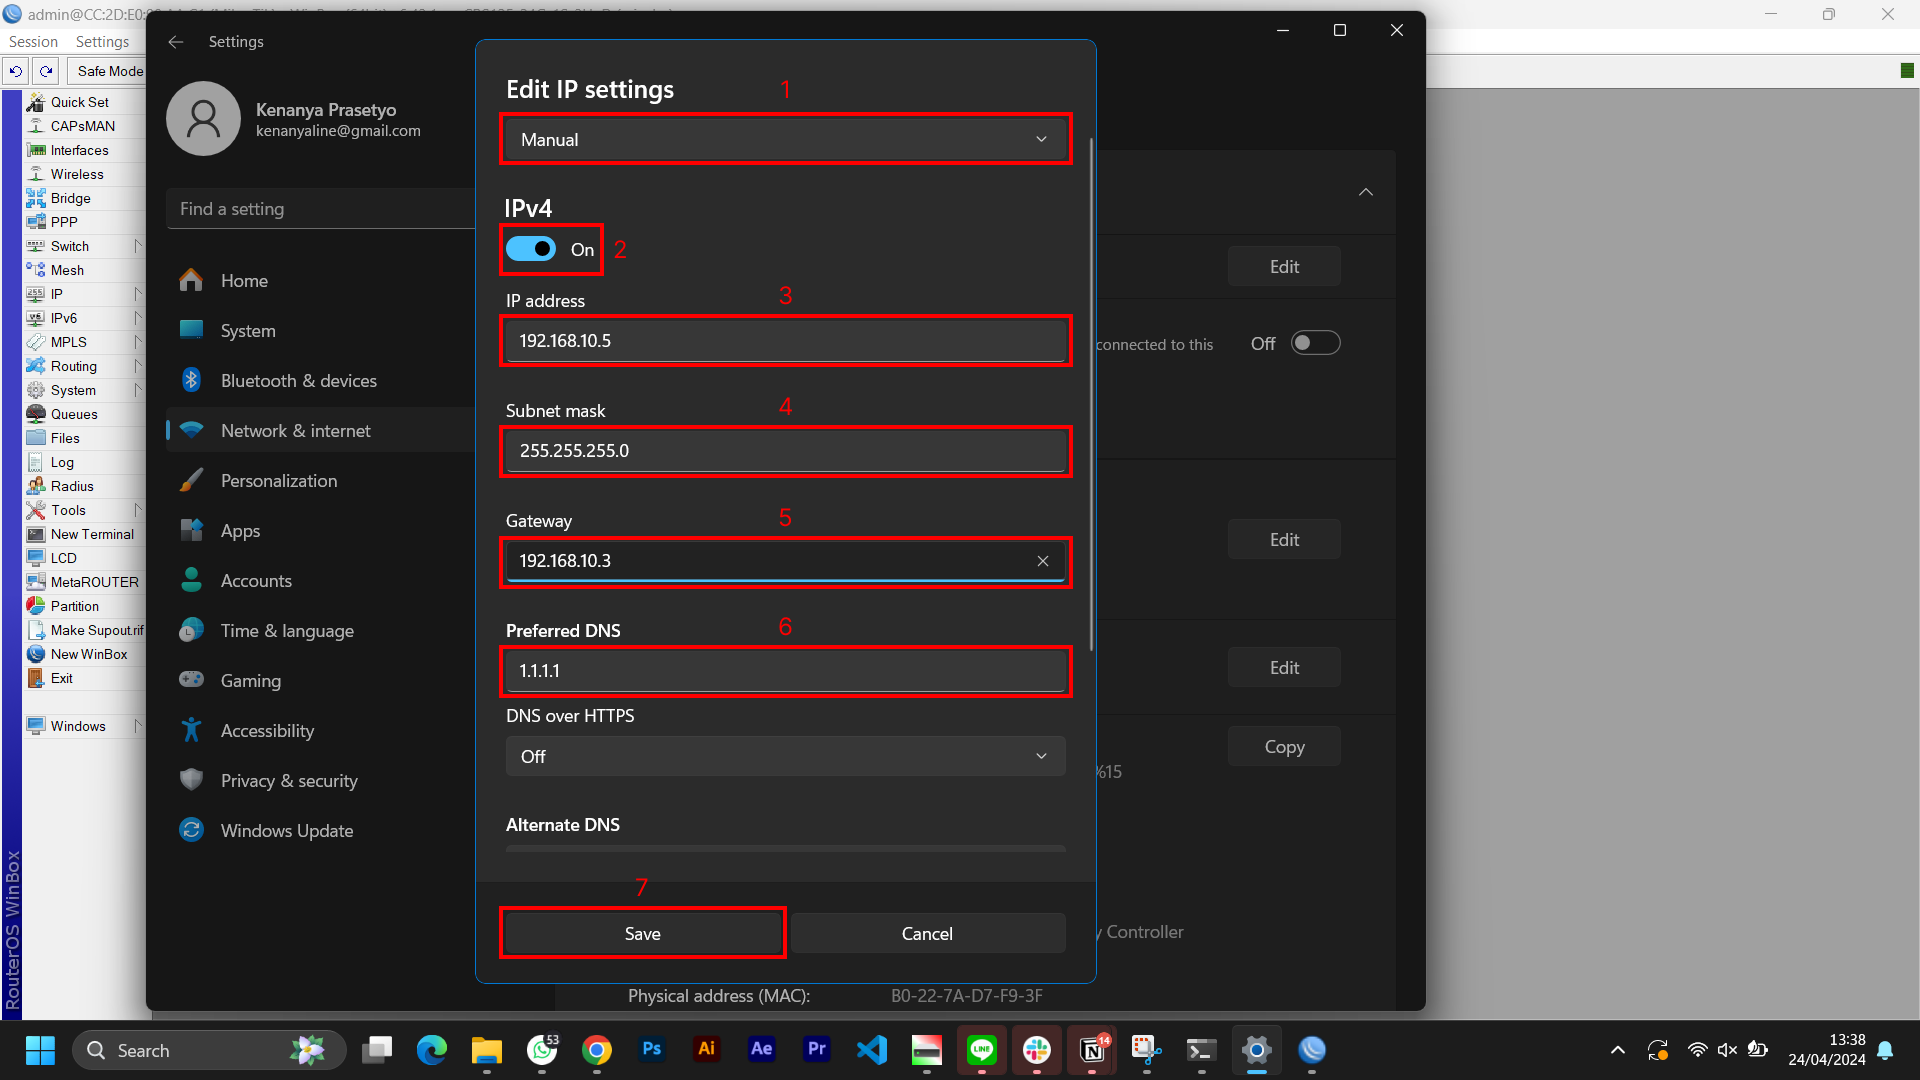
\includegraphics[width=0.9\linewidth]{P1/img/per3/pc2/Step 6.png}
			\caption{Step 6}
			\label{fig:Step 6(Per.3 PC2)}
		\end{figure}
	\end{enumerate}

	\textbf{Mengecek keberhasilan konfigurasi}
	\begin{enumerate}
		\item Lakukan test ping dari PC 1 ke PC 2
		\begin{figure}[H]
			\centering
			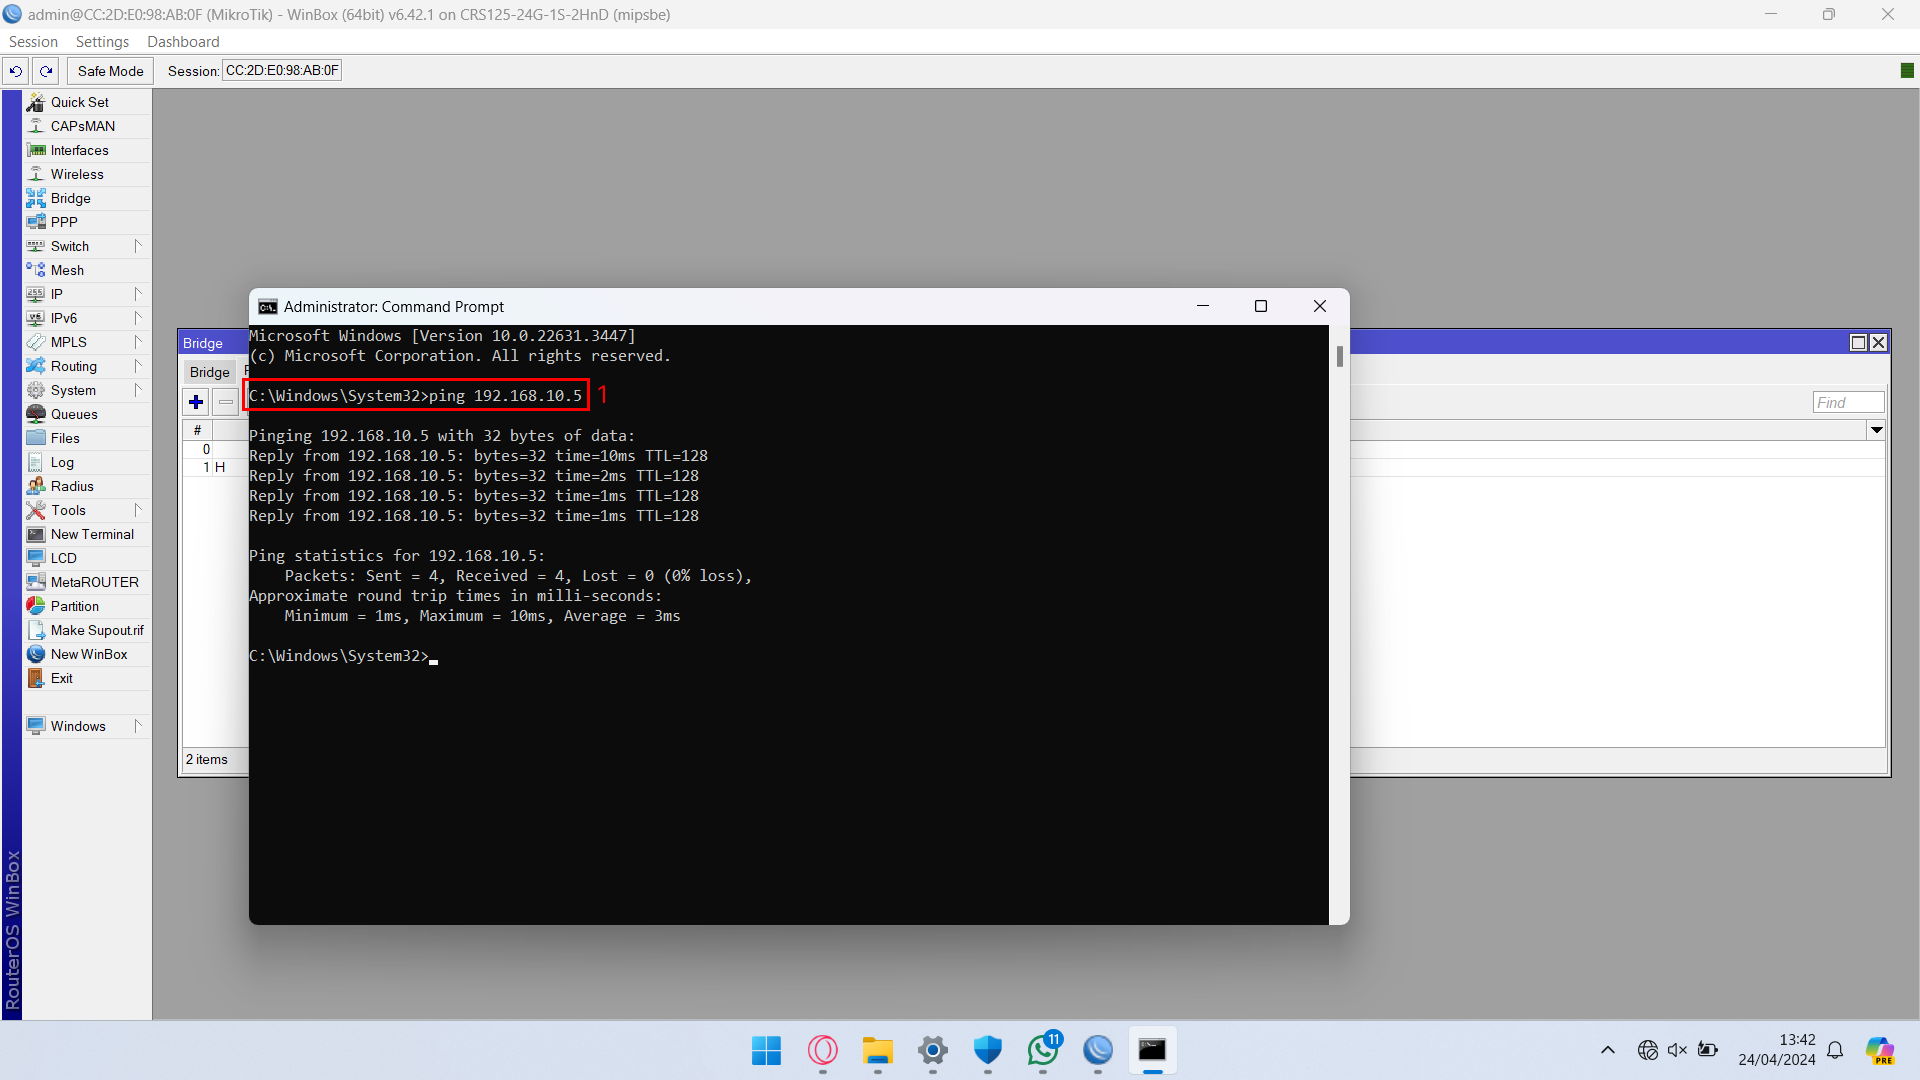
\includegraphics[width=0.9\linewidth]{P1/img/per3/pc1/Step 7.png}
			\caption{Step 7}
			\label{fig:Step 7(Per.3 PC1)}
		\end{figure}
		\item Lakukan test ping dari PC 2 ke PC 1
		\begin{figure}[H]
			\centering
			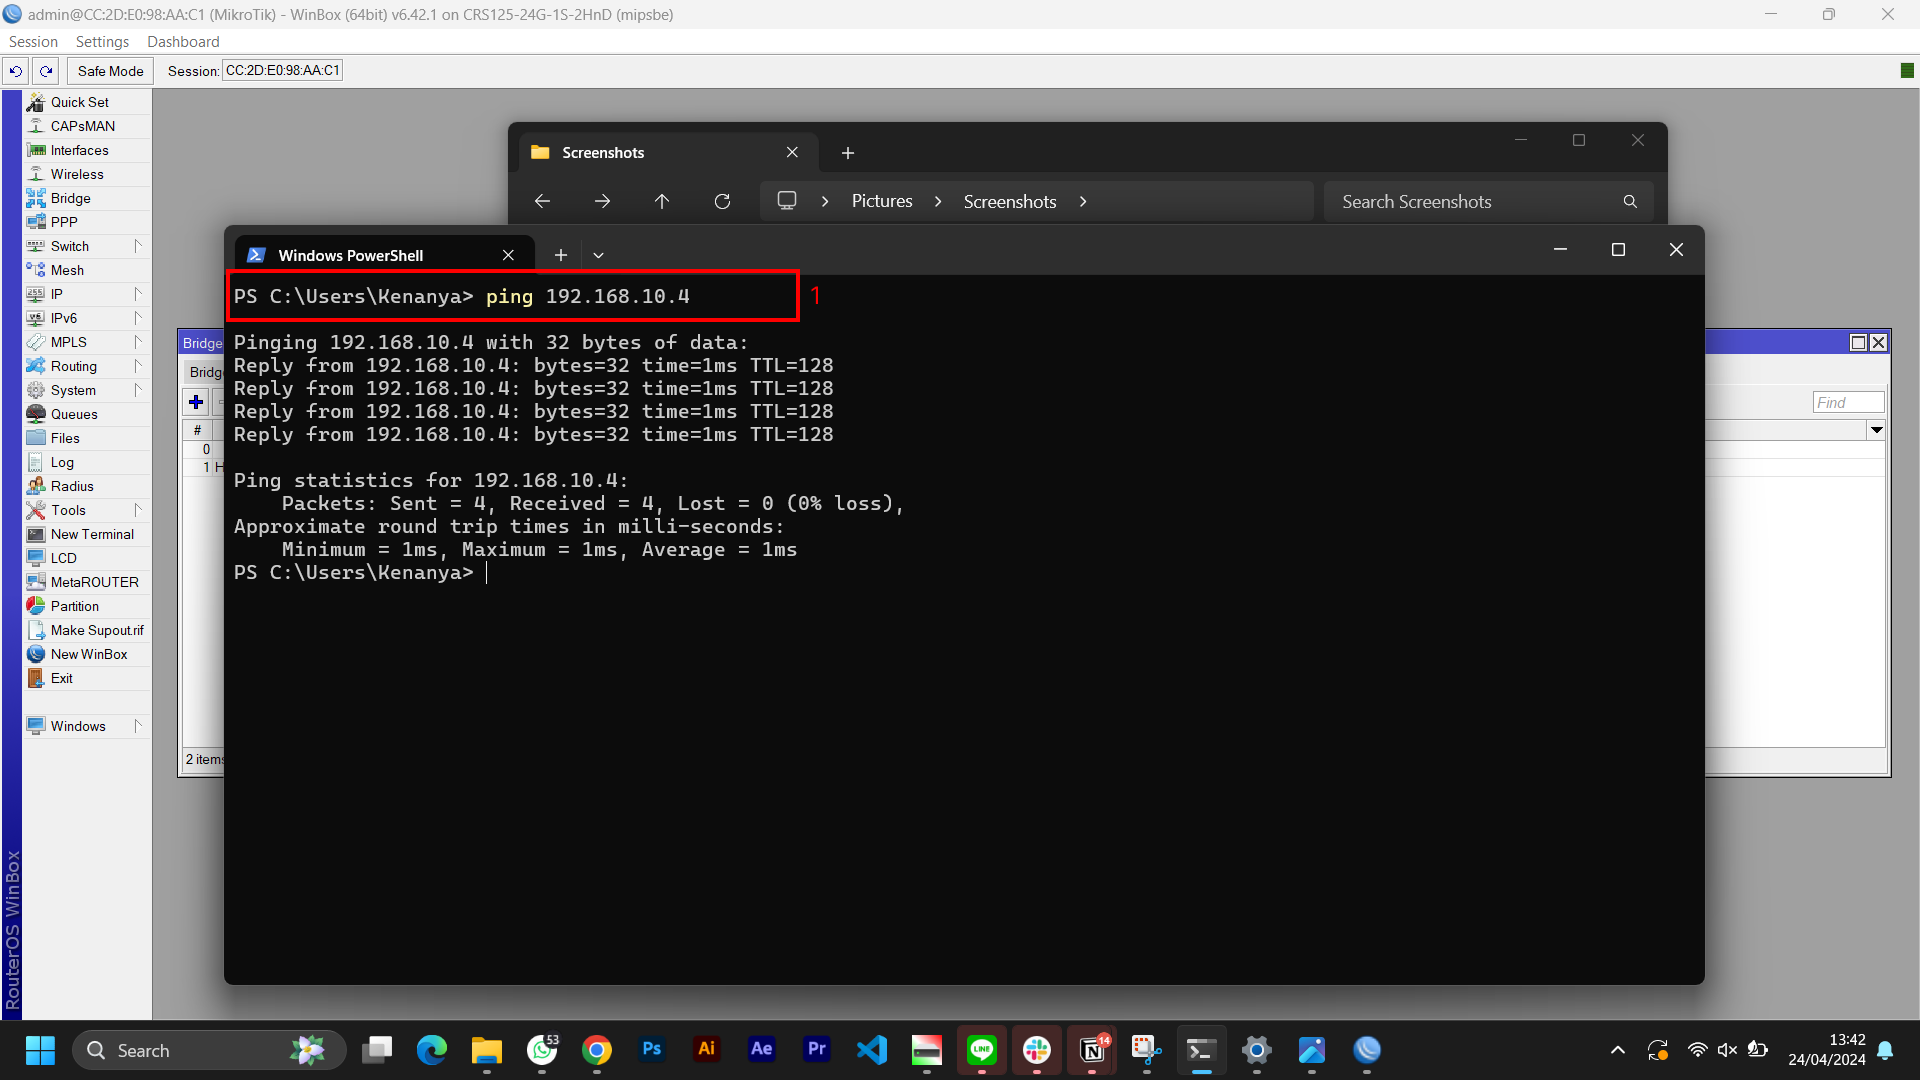
\includegraphics[width=0.9\linewidth]{P1/img/per3/pc2/Step 7.png}
			\caption{Step 7}
			\label{fig:Step 7(Per.3 PC2)}
		\end{figure}
		\item Jika ping antar PC tidak berhasil, coba ulang setelah mematikan Firewall Public PC anda.
	\end{enumerate}
\end{center}

%===========================================================%
\section{Hasil yang didapat}
Memahami dan mengkonfigurasi koneksi Point to Point, Point to Multipoint dan Wireless
Bridging dengan tepat.

%===========================================================%
\section{Temuan Permasalahan}
Firewall hidup pada Laptop dapat mempengaruhi koneksi wireless tidak terhubung, kalian
bisa menonaktifkan firewall di laptop kalian, tetapi hal ini tidak terjadi di semua perangkat.

%===========================================================%
\section{Kesimpulan}
Dengan memahami dan mengkonfigurasi 3 jenis koneksi pada wireless, kita dapat
mengimplementasikan koneksi wireless dengan tepat sesuai kebutuhan dan kondisi tertentu.
